\documentclass{article}
\usepackage[a4paper, total={15cm, 23cm}]{geometry}
\usepackage{float}
\usepackage{tikz}
\usepackage{gensymb}
\usepackage{ulem}
\usepackage{xcolor}
\usepackage{hyperref}
\usepackage{amsmath}
\usepackage{nameref}
\usepackage{pgfplots}
\usepackage[thinlines]{easytable}
\usepackage{array}
\usepackage{circuitikz}
\usepackage{adjustbox}
\usepackage{graphicx}
\usepackage{listings}
\usepackage[utf8]{inputenc}

\tikzstyle{boxes} = [rectangle, minimum width=2cm, minimum height=1cm, text centered, text
width=2cm, draw=black]
\tikzstyle{wboxes} = [rectangle, minimum width=3cm, minimum height=1cm, text centered, text
width=3cm, draw=black]
\tikzstyle{wwboxes} = [rectangle, minimum width=4cm, minimum height=1cm, text centered, text
width=4cm, draw=black]
\tikzstyle{wdiamond} = [diamond, minimum width=3cm, minimum height=1cm, text centered, text
width=3cm, draw=black]
\tikzstyle{xwboxes} = [rectangle, minimum width=8cm, minimum height=1cm, text centered, text
width=8cm, draw=black]
\tikzstyle{square} = [rectangle, minimum width=2cm, minimum height=2cm, text centered, text
width=2cm, draw=black]
\tikzstyle{smboxes} = [rectangle, minimum width=2cm, minimum height=0.75cm, text centered, text
width=2cm, draw=black, line width=1pt, inner sep=0pt, node distance=-1pt]
\tikzstyle{xsmboxes} = [rectangle, minimum width=0.75cm, minimum height=0.75cm, text centered, text
width=0.5cm, draw=black, line width=1pt, inner sep=0pt, node distance=-1pt]
\tikzstyle{line} = [thick, -, >=stealth]
\tikzstyle{arrow} = [thick, ->, >=stealth]
\tikzstyle{dasharrow} = [dashed, ->, >=stealth]
\tikzstyle{darrow} = [thick, <->, >=stealth]

\usetikzlibrary{matrix}
\usetikzlibrary{shapes,snakes}
\usepgfplotslibrary{fillbetween}

\setcounter{tocdepth}{4}
\setcounter{secnumdepth}{4}

\definecolor{codegreen}{rgb}{0,0.6,0}
\definecolor{codegray}{rgb}{0.5,0.5,0.5}
\definecolor{codepurple}{rgb}{0.58,0,0.82}
\definecolor{backcolour}{rgb}{0.95,0.95,0.92}

\lstdefinestyle{codestyle}{
    backgroundcolor=\color{backcolour},   
    commentstyle=\color{codegreen},
    keywordstyle=\color{magenta},
    numberstyle=\tiny\color{codegray},
    stringstyle=\color{codepurple},
    basicstyle=\ttfamily\footnotesize,
    breakatwhitespace=false,         
    breaklines=true,                 
    captionpos=b,                    
    keepspaces=true,                 
    numbers=left,                    
    numbersep=5pt,                  
    showspaces=false,                
    showstringspaces=false,
    showtabs=false,                  
    tabsize=2
}


\lstset{style=codestyle}

\newcommand\todo[1]{\textcolor{red}{\textbf{#1}}}
\newcommand\red[1]{\textcolor{red}{#1}}
\newcommand\green[1]{\textcolor{green}{#1}}
\title{ENCE461 2020 Term 2 Study Notes}

\author{Jos Craw}

\begin{document}
\maketitle
\tableofcontents
\newpage

\section{Debugging}
\begin{itemize}
    \item \textbf{Debugging} Debugging allows the programmer to verify the correctness of a program. The debugger runs the program
    and is able to detect the current state of the program including variable values and register states.

    \item \textbf{Profiling} Profiling collects a time record of the program execution 
\end{itemize}

\textbf{Debugger Types:}
\begin{itemize}
    \item \nameref{section:JTAG}
    \item \nameref{section:SWD}
    \item \nameref{section:OpenOCD}
    \item \nameref{section:GDB}
\end{itemize}

\subsection{JTAG}
\label{section:JTAG}
Joint Test Action Group (JTAG) is a specialized serial bus developed in the 1980s it is defined in the standard IEEE 1491 in 1990.
The main use of this bus is to program and debug microprocessors and other programmable logic devices. This standard provides a test access
port and boundary scan architecture for integrated circuits. \textbf{Boundary Scan Architecture} allows values on pins to be read from and written
to without the use of external tools such as oscilloscopes and signal generators.

\begin{figure}[H]
\begin{adjustbox} {max width=1\textwidth, center}
\centering   
\begin{circuitikz}
    \ctikzset{multipoles/thickness=3}
    \ctikzset{multipoles/dipchip/width=2}

    % U0
    \draw (0, 0) node[dipchip, num pins=8, hide numbers, no topmark,
        external pins width=0](U0) {U0};

    \node [right, font=\tiny] at (U0.bpin 1) {TMS};
    \node [right, font=\tiny] at (U0.bpin 2) {TCK};
    \draw (U0.bpin 2) ++(0, 0.1) -- ++(0.1, -0.1);
    \draw (U0.bpin 2) ++(0, -0.1) -- ++(0.1, 0.1);
    \node [right, font=\tiny] at (U0.bpin 4) {TDI};

    \node [left, font=\tiny] at (U0.bpin 5) {TDO};

    % U1
    \draw (5, 0) node[dipchip, num pins=8, hide numbers, no topmark,
    external pins width=0](U1) {U1};

    \node [right, font=\tiny] at (U1.bpin 1) {TMS};
    \node [right, font=\tiny] at (U1.bpin 2) {TCK};
    \draw (U1.bpin 2) ++(0, 0.1) -- ++(0.1, -0.1);
    \draw (U1.bpin 2) ++(0, -0.1) -- ++(0.1, 0.1);
    \node [right, font=\tiny] at (U1.bpin 4) {TDI};

    \node [left, font=\tiny] at (U1.bpin 5) {TDO};

    % U2
    \draw (10, 0) node[dipchip, num pins=8, hide numbers, no topmark,
    external pins width=0](U2) {U2};

    \node [right, font=\tiny] at (U2.bpin 1) {TMS};
    \node [right, font=\tiny] at (U2.bpin 2) {TCK};
    \draw (U2.bpin 2) ++(0, 0.1) -- ++(0.1, -0.1);
    \draw (U2.bpin 2) ++(0, -0.1) -- ++(0.1, 0.1);
    \node [right, font=\tiny] at (U2.bpin 4) {TDI};

    \node [left, font=\tiny] at (U2.bpin 5) {TDO};

    % Drawing the connections
    \node [left] at (-4, 3) {TMS};
    \node [left] at (-4, 2) {TCK};
    \node [left] at (-4, 52 |- U0.bpin 4) {TDI};
    \node [left] at (-4, -2) {TDO};


    \node[circ] at (-2, 3) {};
    \node[circ] at (-2.5, 2) {};
    \node[jump crossing] at (-2, 2) (cr0) {};
    \draw (-4, 3) -- (-2, 3);
    \draw (-4, 2) -- (-2.5, 2);
    \draw (-2.5,  2) -- (cr0.west);
    \draw (-2, 3) |- (U0.bpin 1);
    \draw (-2.5, 2) |- (U0.bpin 2);
    \draw (-4, 52 |- U0.bpin 4) -- (U0.bpin 4);
    \draw (U0.bpin 5) -- (U1.bpin 4);

    \node[circ] at (3, 3) {};
    \node[circ] at (2.5, 2) {};
    \node[jump crossing] at (3, 2) (cr1) {};
    \draw (-2, 3) -- (3, 3);
    \draw (cr0.east) -- (cr1.west);
    \draw (3, 3) |- (U1.bpin 1);
    \draw (2.5, 2) |- (U1.bpin 2);
    \draw (U1.bpin 5) -- (U2.bpin 4);

    \draw (3, 3) -- (8, 3);
    \draw (cr1.east) -- (7.5, 2);
    \draw (8, 3) |- (U2.bpin 1);
    \draw (7.5, 2) |- (U2.bpin 2);
    \draw (U2.bpin 5) -| (12, -2);
    \draw (12, -2) -- (-4, -2);

\end{circuitikz}
\end{adjustbox}
\caption{Daisy Chained JTAG Ports}
\label{fig:jtag}
\end{figure}


JTAG contains the following possible signals:
\begin{enumerate}
    \item \textbf{TCK} - Test Clock for clocking test data entering on TDI and TDO
    \item \textbf{TMS} - Test mode state: frame sync and JTAG mode switch
    \item \textbf{TDI} - Test data in
    \item \textbf{TDO} - Test data out
    \item \textbf{TRST} - Test reset (\textit{optional}, 4+1 interface) to reset the test
\end{enumerate}

\subsection{SWD}
\label{section:SWD}
Single Wire Debug (SWD) is a debug port for pin limited packages, it is a 2+1 pin arrangement vs JTAG 4+1 arrangement. The first pin is used for
clock (\textbf{SWCLK}) with is equivalent to TCK and TMS on JTAG. The other pin (\textbf{SWDIO}) is equivalent to TDI and TDO on JTAG and handles
data transmission. SWD is the ARM standard bi-directional wire protocal and is defined in the ARM Debug interface v5 and can transmit data to and from the
debugger and target board without target-resident code, it is also compatible with all ARM processors. Standard modules provide all normal JTAG debug and test 
functionality as well as power. This system uses synchronous bi-directional transmission, simmilar to $\textrm{I}^2\textrm{C}$.

\subsection{OpenOCD}
\label{section:OpenOCD}
OpenOCD runs a server with is accessible through a terminal on port 4444 and accessible to GDB through port 3333.

\begin{figure}[H]
    \begin{center}
        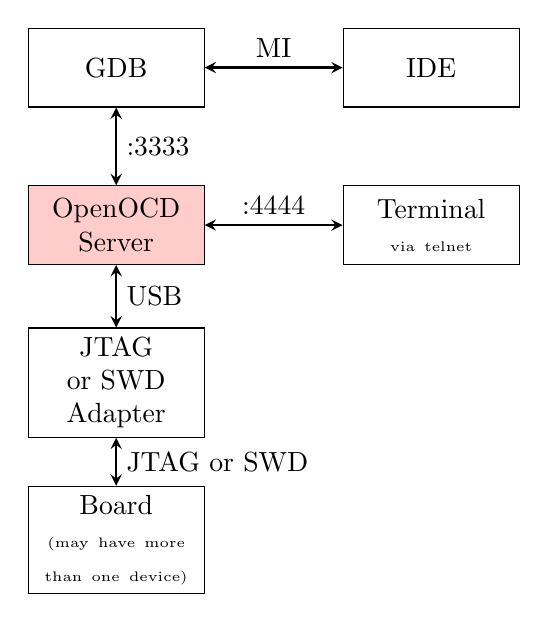
\begin{tikzpicture}
            % Draw Boxes
            \node(gdb) [boxes] {GDB};
            \node(ide) [boxes, right of=gdb, xshift=3cm] {IDE};
            \node(oocd) [boxes, below of=gdb, fill=red!20, yshift=-1cm] {OpenOCD Server};
            \node(terminal) [boxes, right of=oocd, xshift=3cm] {Terminal\\{\tiny via telnet}};
            \node(jtag) [boxes, below of=oocd, yshift=-1cm] {JTAG or SWD Adapter};
            \node(board) [boxes, below of=jtag, yshift=-1cm] {Board\\{\tiny (may have more than one device)}};

            % Draw Arrows
            \draw[darrow] (gdb) -- (ide) node[midway, above] {MI};
            \draw[darrow] (gdb) -- (oocd) node[midway, right] {:3333};
            \draw[darrow] (oocd) -- (terminal) node[midway, above] {:4444};
            \draw[darrow] (oocd) -- (jtag) node[midway, right] {USB};
            \draw[darrow] (jtag) -- (board) node[midway, right] {JTAG or SWD};
        \end{tikzpicture}
    \end{center}
    \caption{OpenOCD Access structure}
    \label{fiog:openocd}
\end{figure}

\subsection{GDB}
\label{section:GDB}
GDB is a command line debugger in Unix and Linux and is supported under OpenOCD. There is not always a GUI available for the software.\\

The following commands run GDB:
\vspace{0.5cm}

\begin{figure}[H]
\begin{center}
\begin{lstlisting}[language=bash]
gdb $EXE_NAME
gdb -e $EXE_NAME -c $CORE_FILE_NAME
gdb $EXE_NAME --pid=$PROCESS_ID
\end{lstlisting}
\end{center}
\caption{Unix commands to invoke the GDB Debugger}
\label{fig:unix-commands}
\end{figure}


\section{Startup Procedure}
\subsection{Memory Sections}
A program for an embedded system generally consists of more than one source file.
After compilation these files are organised into different memory sections:

\begin{itemize}
    \item \textbf{.text} - Code and instructions
    \item \textbf{.rodata} - Constraints {\small (eg. pi cosine/sine tables, FIR filter coefficients etc.)}
    \item \textbf{.data} - Initialised Data {\small (Global, static and local variables with initial values)}
    \item \textbf{.bss} - Uninitialised Data {\small {Global, static and local variables that are uninitialised or initialised to 0}}
\end{itemize}

The \textbf{.text}, \textbf{.rodata} and \textbf{.data} segments all are held within flash memory as they casn be fetched when required and
do not need to be held in SRAM.\\

The \textbf{.data} and \textbf{.bss} are held within SRAM as they may change with ht program therefore SRAM is the most suitable.\\

\textbf{NOTE:} The \textbf{.data} segment can be held within both, this is because initialised variables may be changed throughout
the course of a program run and therefore maybe moved to SRAM.\\

As shown in Figure \ref{fig:mem-stack} the heap and the stack typically grow toward each other.

\begin{figure}[H]
    \begin{center}
        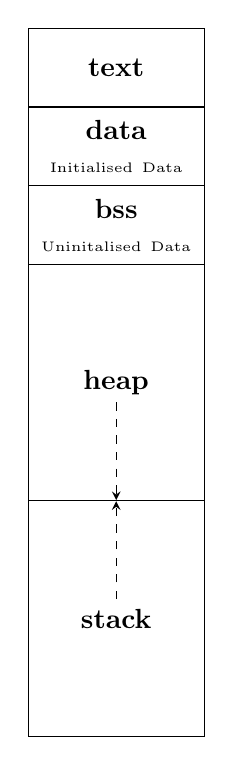
\begin{tikzpicture}
            \node(text) [boxes] {\textbf{text}};
            \node(data) [boxes, below of=text] {\textbf{data}\\{\tiny Initialised Data}};
            \node(bss) [boxes, below of=data] {\textbf{bss}\\{\tiny Uninitalised Data}};
            \node(heap) [boxes, below of=bss, minimum height=3cm, yshift=-1cm] {\textbf{heap}};
            \node(stack) [boxes, below of=heap, minimum height=3cm, yshift=-2cm] {\textbf{stack}};
            \draw[dasharrow] (0, -4.25) -- (stack);
            \draw[dasharrow] (0, -6.75) -- (heap);
        \end{tikzpicture}
    \end{center}
    \caption{Memory Stack}
    \label{fig:mem-stack}
\end{figure}

\textbf{Heap}, the heap contains dynamic memory allocations, this area is what is provided when
malloc(), calloc(), realloc() and free() are called in C. The heap starts at the bottom of the bss section 
and grows down toward the stack.\\

\textbf{Stack}, the stack has a Last in First out (LIFO) structure and starts at the end of SRAM and grows
toward smaller address numbers.

\subsection{Linking}
Linking is the mapping of certain sections of physical memory to virtual memory space.

\begin{itemize}
    \item Code and Constraints (.text and .rodata) $\to$ FLASH {\tiny (Read Only)}
    \item Uninitialised variables (.bss) $\to$ SRAM {\tiny (Read Write)}
    \item Initialised variables (.data) $\to$ FLASH and SRAM {\tiny (copy data before runtime for both read and write)}
    \item Interrupt vector table $\to$ start of FLASH
\end{itemize}

\subsubsection{Memory Map}

\begin{figure}[H]
    \begin{center}
        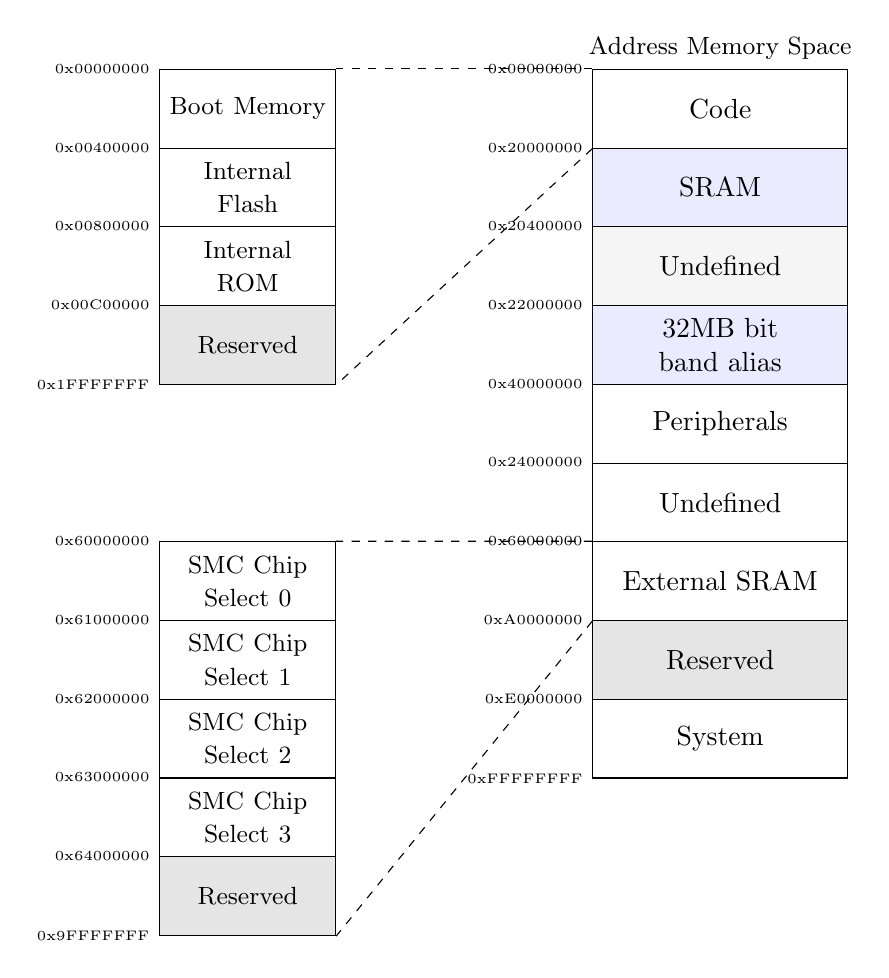
\begin{tikzpicture}
            \node(code) [wboxes] {Code};
            \node(sram) [wboxes, below of=code, fill=blue!8] {SRAM};
            \node(undefined) [wboxes, below of=sram, fill=gray!8] {Undefined};
            \node(bitband) [wboxes, below of=undefined, fill=blue!8] {32MB bit band alias};
            \node(periph) [wboxes, below of=bitband] {Peripherals};
            \node(undef1) [wboxes, below of=periph] {Undefined}; 
            \node(externalsram) [wboxes, below of=undef1] {External SRAM};
            \node(reserved) [wboxes, below of=externalsram, fill=gray!20] {Reserved};
            \node(system) [wboxes, below of=reserved] {System};

            % Address stuff
            \draw node[left] at (code.north west) {\tiny 0x00000000};
            \draw node[left] at (sram.north west) {\tiny 0x20000000};
            \draw node[left] at (undefined.north west) {\tiny 0x20400000};
            \draw node[left] at (bitband.north west) {\tiny 0x22000000};
            \draw node[left] at (undef1.north west) {\tiny 0x24000000};
            \draw node[left] at (periph.north west) {\tiny 0x40000000};
            \draw node[left] at (externalsram.north west) {\tiny 0x60000000};
            \draw node[left] at (reserved.north west) {\tiny 0xA0000000};
            \draw node[left] at (system.north west) {\tiny 0xE0000000};
            \draw node[left] at (system.south west) {\tiny 0xFFFFFFFF};

            \draw node[above] at (code.north) {\small Address Memory Space};
            
            % Draw Code sub memory
            \node(bootmem) [boxes, left of=code, xshift=-5cm] {\small Boot Memory};
            \node(intflash) [boxes, below of=bootmem] {\small Internal Flash};
            \node(introm) [boxes, below of=intflash] {\small Internal ROM};
            \node(reserv) [boxes, below of=introm, fill=gray!20] {\small Reserved};

            % Draw Labels
            \draw node[left] at (bootmem.north west) {\tiny 0x00000000};
            \draw node[left] at (intflash.north west) {\tiny 0x00400000};
            \draw node[left] at (introm.north west) {\tiny 0x00800000};
            \draw node[left] at (reserv.north west) {\tiny 0x00C00000};
            \draw node[left] at (reserv.south west) {\tiny 0x1FFFFFFF};

            % Draw Lines
            \draw[dashed] (code.north west) -- (bootmem.north east);
            \draw[dashed] (code.south west) -- (reserv.south east);

            % Draw external RAM sub memory
            \node(smc0) [boxes, below of=reserv, yshift=-2cm] {\small SMC Chip Select 0};
            \node(smc1) [boxes, below of=smc0] {\small SMC Chip Select 1};
            \node(smc2) [boxes, below of=smc1] {\small SMC Chip Select 2};
            \node(smc3) [boxes, below of=smc2] {\small SMC Chip Select 3};
            \node(res) [boxes, below of=smc3, fill=gray!20] {\small Reserved};

            % Draw Labels
            \draw node[left] at (smc0.north west) {\tiny 0x60000000};
            \draw node[left] at (smc1.north west) {\tiny 0x61000000};
            \draw node[left] at (smc2.north west) {\tiny 0x62000000};
            \draw node[left] at (smc3.north west) {\tiny 0x63000000};
            \draw node[left] at (res.north west) {\tiny 0x64000000};
            \draw node[left] at (res.south west) {\tiny 0x9FFFFFFF};

            % Draw Lines
            \draw[dashed] (externalsram.north west) -- (smc0.north east);
            \draw[dashed] (externalsram.south west) -- (res.south east);

            
        \end{tikzpicture}
    \end{center}
    \caption{Memory Mappings}
    \label{fig:mem-map}
\end{figure}


From Figure \ref{fig:mem-map}:

\begin{itemize}
    \item The system always boots at 0x00000000
    \item Internal ROM from 0x080000000 contains:
        \begin{itemize}
            \item SAM boot assistant
            \item In-application programming (IAP) routines
            \item Fast FLASH programming interface (FFPI)
            \item Easy way for programming \todo{in-situ} the on chip FLASH memory via serial communication UART/USB SAM-BA GUI provided
        \end{itemize}
    \item Internal Flash, first address contains the interrupt register
    \item Boot using SAM-BAon the ROM (\textit{default})
        \begin{itemize}
            \item General Purpose NVM (GPNVM) bit=0
        \end{itemize}
    \item Boot using SAM-BA on FLASH
        \begin{itemize}
            \item General-purpose NVM (GPNVM) bit=1
        \end{itemize}
    \item Enhanced embedded FLASH controller (EEFC) user interface: set GPNVM bit
\end{itemize}

\subsection{Linker Script}
\begin{itemize}
    \item MEMORY Figure \ref{fig:linker-mem}
    \item SECTIONS Figure \ref{fig:linker-sections}
    \item .text Figure \ref{fig:linker-text}
    \item .data Figure \ref{fig:linker-data}
\end{itemize}
Firstly, this linker script specifies the memory space according to the previously defined memory map.

\begin{figure}[H]
    \begin{center}
    \begin{lstlisting}[language=C]
    MEMORY
    {
        FLASH (rx) : ORIGIN = 0x00400000, LENGTH = 1M
        SRAM (rwx) : ORIGIN = 0x20000000, LENGTH = 128K
    }
    \end{lstlisting}
    \end{center}
    \caption{Linker Script memory declaration}
    \label{fig:linker-mem}
\end{figure}

Where, FLASH is readable and executable `(rx)' and SRAM is readable, writable and executable `(rwx)'\\

Next, physical memory addresses are specified for sections as shown in Figure \ref{fig:linker-sections}

\begin{figure}[H]
    \begin{center}
    \begin{lstlisting}[language=C]
    SECTIONS
    {
        . = 0x0000000; // `.' is the location counter
        /* ... */
    }
    \end{lstlisting}
    \end{center}
    \caption{Linker Script Section declaration}
    \label{fig:linker-sections}
\end{figure}

All of the \textbf{.text} sections from all of the object files are combined into a single \textbf{.text} section with
the following script.

\begin{figure}[H]
    \begin{center}
    \begin{lstlisting}[language=C]
    .text :
    {
        /* .text section starts with an address with the last two bits = `00' */
        . = ALIGN(4); 
        /* Concatenate all .text sections */
        *(.text)
    } >FLASH // Put the .text section in FLASH
    \end{lstlisting}
    \end{center}
    \caption{Linker Script Section declaration}
    \label{fig:linker-text}
\end{figure}

The \textbf{.data} sections are loaded into FLASH and SRAM at startup

\begin{figure}[H]
    \begin{center}
    \begin{lstlisting}[language=C]
    .data : AT (__text_end__)
    {
        __data_start__ = .;
        *(.data)
        __data_end__ = .;
        __data_load__ = LOADADDR (.data); // Returns load memory address of .data section
    } >SRAM // Put the .data section in SRAM

    /*
        AT is the starting load memory address of the .data section in FLASH
        __data_start__, __data_end__ and _  __data_load__ are SRAM addresses
    */
    \end{lstlisting}
    \end{center}
    \caption{Linker Script Section declaration}
    \label{fig:linker-data}
\end{figure}

\subsection{Boot from RESET}
The SAM4S clock initally runs off of the internal 4MHz RC oscillator\\
On RESET the the SAM4S loads the program counter (PC) with the address of the RESET interrupt service routine (ISR)\\

The following code Figure \ref{fig:boot-reset} describes the reset handler:
\begin{figure}[H]
    \begin{center}
    \begin{lstlisting}[language=C]
    void _reset_handler(void) {
        /* Init the preinitialised variables in .data */
        for (char *src = & __data_load__, char *dst = &__data_start__; dst < &__data_end__) {
            *dst++ = *src++;
        }

        /* Zero all remaining uninitialised global variables in .bss */
        for (dst = &__bss_start__; dst < &__bss_end__; ) {
           *dst++ = 0;
        }

        /* 
        Remap the exception table into SRAM to allow dynamic 
        allocation. This register is zero on reset 
        */
        SCB->VTOR = (uint32_t)&exception_table & SCB_VTOR_TBLOFF_Msk;

        /* Set up clockes, etc. */
        mcu_init();

        main();

        /* Hang on program termination */
        while (1) { continue; }
    }
    \end{lstlisting}
    \end{center}
    \caption{Reset Handler code snippet}
    \label{fig:boot-reset}
\end{figure}


\begin{figure}[H]
    \begin{center}
    \begin{lstlisting}[language=C]
    void mcu_init(void) {
        /* Disable all interrupts */
        for (int i = 0; i < 8; i++) {
            /* 
            ICER0 - ICER7: 32 bit vector indicating the 
            enabled/disabled interrupts 
            */
            NVIC->ICER[i] = ~0;
        }

        mcu_reset_enable();

        /* Reduce the number of wait states for the flash memory */
        mcu_flash_init();

        mcu_watchdog_disable();
        mcu_clock_init();
        irq_global_enable();
    }
    \end{lstlisting}
    \end{center}
    \caption{MCU initialisation code snippet}
    \label{fig:boot-mcu-init}
\end{figure}



\section{Serial Interfaces}
\subsection{Serial interfaces vs parallel interfaces}
\begin{itemize}
    \item Serial interfaces
        \begin{itemize}
            \item Encode bits by their temporal locations in the transmission medium
            \item Suitable for pin-limited devices
        \end{itemize}
    \item Parallel interfaces
    \begin{itemize}
        \item Encoded use spacial locality
    \end{itemize}
    \item Issues
    \begin{itemize}
        \item How does the device know when to start looking for information?
        \item What is the bit order?
        \item How does the receiver know when the transmission is complete?
    \end{itemize}
\end{itemize}

\subsection{Simplex, Full-Duplex and Half-Duplex}
\begin{figure}[H]
    \begin{center}
        \begin{circuitikz}
            % Simplex
            \draw node[buffer] (sim0) at (0, 0) {};
            \draw node[buffer] (sim1) at (4, 0) {};
            \draw (sim0.out) -- (sim1.in) node[above, midway, yshift=1cm] {{\large Simplex} {\small (One direction)}};
            \draw (sim0.in) -- ++(-1, 0);
            \draw (sim1.out) -- ++(1, 0);

            % Half Duplex
            \draw node[buffer] (hdup0) at (-1, -3) {};
            \draw node[buffer, rotate=180] (hdup1) at (-1, -4) {};

            \draw node[buffer] (hdup2) at (5, -3) {};
            \draw node[buffer, rotate=180] (hdup3) at (5, -4) {};

            \draw node[spdt, rotate=180] (sw0) at (1, -3.5) {};
            \draw node[spdt] (sw1) at (3, -3.5) {};

            \draw (hdup0.in) -- ++(-1, 0);
            \draw (hdup1.out) -- ++(-1, 0);
            \draw (hdup2.out) -- ++(1, 0);
            \draw (hdup3.in) -- ++(1, 0);

            \draw (hdup0.out) -| (sw0.out 2);
            \draw (hdup1.in) -| (sw0.out 1);
            \draw (hdup2.in) |- (sw1.out 1);
            \draw (hdup3.out) |- (sw1.out 2);

            \draw (sw0.in) -- (sw1.in) node[above, midway, yshift=1.25cm] {{\large Half Duplex} {\small (Both directions one at a time)}};

            % Full Duplex
            \draw node[buffer] (dup0) at (0, -7) {};
            \draw node[buffer] (dup1) at (4, -7) {};
            \draw (dup0.out) -- (dup1.in) node[above, midway, yshift=1cm] {{\large Full Duplex} {\small (Both directions simultaneously)}};
            \draw (dup0.in) -- ++(-1, 0);
            \draw (dup1.out) -- ++(1, 0);

            \draw node[buffer, rotate=180] (dup2) at (0, -8) {};
            \draw node[buffer, rotate=180] (dup3) at (4, -8) {};
            \draw (dup2.out) -- ++(-1, 0);
            \draw (dup3.in) -- ++(1, 0);
            \draw (dup2.in) -- (dup3.out);
        \end{circuitikz}
    \end{center}
    \caption{Simplex vs Full Duplex vs Half Duplex}
    \label{fig:sim-vs-duplex}
\end{figure}

\subsection{Asynchronous vs Synchronous}

\noindent \textbf{NOTE}: This is NOT required for analogue communications.

\begin{itemize}
    \item Asynchronous
    \begin{itemize}
        \item No clock signal transmitted
        \item Each end has a clock with the same \textit{nominal} frequency
        \item Clock and frame synchronization is required
    \end{itemize}
    \item Synchronous
    \begin{itemize}
        \item Clock is sent over a separate wire
        \item Clock signal is encoded within data (eg. Manchester Code)
    \end{itemize}
\end{itemize}

\subsection{Manchester Code}
With non-return to zero (NRZ) coding, clock synchronization would be difficult during long sequences
of either `1' of `0'. Manchester Code negates this by using the voltage transition to represent `1'
and `0'.
\begin{figure}[H]
    \begin{center}
        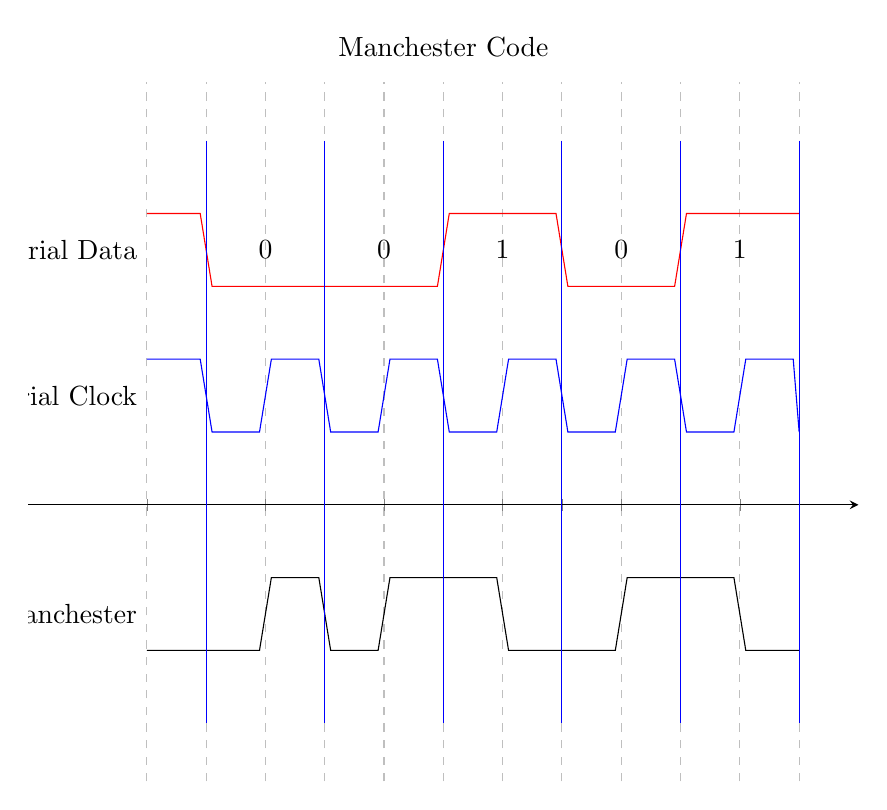
\begin{tikzpicture}
        \begin{axis} [
            width=\textwidth,
            axis x line=middle,
            axis y line=none,
            xmin=-20,
            xmax=120,
            xmajorgrids=true,
            grid style=dashed,
            xtick={0, 10, ..., 110},
            samples=1050,
            title=Manchester Code,
            xticklabels=\empty,
        ]
        
        % Serial Data
        \addplot[red] coordinates
        {(0,4) (9,4) (11,3) (49,3) (51,4) (69,4) (71,3) (89,3) (91,4) (110,4)};

        % Serial Clock
        \addplot[blue] coordinates
        {(0,2) (9,2) (11,1) (19,1) (21,2) (29,2) (31,1) (39,1) (41,2) (49,2) (51,1) (59,1) (61,2)
        (69,2) (71,1) (79,1) (81,2) (89,2) (91,1) (99, 1) (101, 2) (109,2) (110,1)};

        % Manchester
        \addplot[black] coordinates
        {(0,-2) (19,-2) (21,-1) (29,-1) (31,-2) (39,-2) (41,-1) (59,-1) (61,-2) (79,-2) (81,-1)
        (99,-1) (101,-2) (110,-2)};

        % Vertical Lines
        \addplot[blue] coordinates
        {(10,5) (10,-3)};
        \addplot[blue] coordinates
        {(30,5) (30,-3)};
        \addplot[blue] coordinates
        {(50,5) (50,-3)};
        \addplot[blue] coordinates
        {(70,5) (70,-3)};
        \addplot[blue] coordinates
        {(90,5) (90,-3)};
        \addplot[blue] coordinates
        {(110,5) (110,-3)};

        % Serial Data
        \node[] at (axis cs:20,3.5) {0};
        \node[] at (axis cs:40,3.5) {0};
        \node[] at (axis cs:60,3.5) {1};
        \node[] at (axis cs:80,3.5) {0};
        \node[] at (axis cs:100,3.5) {1};

        % Signal Labels
        \node[left] at (axis cs:0,3.5) {Serial Data};
        \node[left] at (axis cs:0,1.5) {Serial Clock};
        \node[left] at (axis cs:0,-1.5) {Manchester}; 
        \end{axis}
        \end{tikzpicture}
    \end{center}
    \caption{Manchester Code of `00101' serial data stream}
    \label{fig:manchester-code}
\end{figure}


\subsection{Serial Interface Comparison}
\begin{table}[H]
\caption{Technical comparison of different serial interfaces}
\label{table:serial-interface}
    \begin{center}
        \begin{tabular} { | m{4cm} | m{1cm} | m{1cm} | m{2.5cm} | m{1cm} | m{1cm} | m{1.5cm} | }
        \hline
        Interface & Sync. & Duplex & Wires & Mode & Topo. & Format\\
        \hline
        UART (RS232) & A & F & 2 + GND & SE & P & NRZ\\
        UART (RS423) & A & F & 2 + GND & SE & M & NRZ\\
        UART (RS422) & A & F & 4 + GND & D & M & NRZ\\
        UART (RS485) & A & F & 4 + GND & D & B & NRZ\\
        $\textrm{Synchronous}^{(1)}$ & S & F & 6 + GND & SE & P & NRZ\\
        SPI & S & F & 3 + GND & SE & M & NRZ\\
        JTAG & S & F & 4 + GND & SE & DC & NRZ\\
        I$^2$C/TWI & S & H & 2 + GND & SE & B & NRZ\\
        CAN & A & H & 2 + GND & D & B & NRZ-BS\\
        LIN & A & H & 1 + GND & S & B & NRZ\\
        Ethernet 100Base-T & S & F & $4$ & D & SH & MPE\\
        USB & A & H & 2 + GND/PWR & D & SH & NRZI-BS\\
        IEEE 1394 {\small (Firewire)} & S & F & 4 + GND/PWR & D & SH & DS\\
        Serial ATA & S & F & 4 + 3 GND & D & P & NRZ\\
        \hline
        \multicolumn{7}{l}{A = Asynchronous}\\
        \multicolumn{7}{l}{S = Synchronous}\\
        \multicolumn{7}{l}{F = Full duplex}\\
        \multicolumn{7}{l}{H = Half Duplex}\\
        \multicolumn{7}{l}{PWR = Power}\\
        \multicolumn{7}{l}{SE = Single ended {\small (Voltage signal with reference to ground)}}\\
        \multicolumn{7}{l}{D = Differential {\small (Complementary Signals)}}\\
        \multicolumn{7}{l}{P = Point to point}\\
        \multicolumn{7}{l}{M = Multipoint}\\
        \multicolumn{7}{l}{B = Bus}\\
        \multicolumn{7}{l}{DC = Daisy chain}\\
        \multicolumn{7}{l}{SH = Switch Hub}\\
        \multicolumn{7}{l}{NRZ = Non-return to zero}\\
        \multicolumn{7}{l}{NRZI = NRZ inverted}\\
        \multicolumn{7}{l}{DS = Data strobe}\\
        \end{tabular}
    \end{center}
\end{table}

\begin{table}[H]
    \caption{Application comparison of serial interfaces}
    \label{table:serial-app-comp}
    \begin{center}
        \begin{tabular} { | m{3cm} | m{2cm} | m{2cm} | m{2cm} | m{5cm} | }
        \hline
        Interface & Max \# Devices & Max Length (feet) & Max Speed (bps) & Application\\
        \hline
        USB (v1.0 \& v2.0) & 127 & 16 & 12M \& 480M & Human interface devices eg. mouse, keyboard\\
        \hline
        RS-232 & 2 & 50-100 & 20k & Modems/Terminals\\
        \hline
        RS-485 & 32 & 4000 & 10M & Data Acquisition, control systems\\
        \hline
        IrDA & 2 & 50-100 & 115k & Printers, hand-held computers\\
        \hline
        SPI & 8 & 10 & 2M [sic] $<$10M (device specific) & Microcontroller peripherals, EEPROM
        memory\\
        \hline
        $\textrm{I}^2\textrm{C}$ & 40 & 18 & 3.4M & As above\\
        \hline
        IEEE-1394 {\small (Firewire v(a) \& v(b))} & 64 & 15 & 400M, 800M & Video, mass storage
        systems\\
        \hline
        Ethernet & 1024 & 1600 & 10M / 100M / 1G / 2.5G / 5G / 10G / 100G & Networking\\
        \hline
        \end{tabular}
    \end{center}
\end{table}


\begin{figure}[H]
    \begin{center}
        \begin{tikzpicture}
            \node(top) [] {MCU Interfaces};
            \node(digital) [below of=top, yshift=-1cm, xshift=-4cm] {Digital};
            \node(analog) [below of=top, yshift=-1cm, xshift=4cm] {Analog};

            % Digital
            \node(on-off) [below of=digital, yshift=-1cm, xshift=-2cm] {On/Off};
            \node(parallel) [below of=digital, yshift=-1cm] {Parallel};
            \node(serial) [below of=digital, yshift=-1cm, xshift=2cm] {Serial};
            \node(async) [below of=serial, yshift=-1cm, xshift=-2cm] {Async.};
            \node(sync) [below of=serial, yshift=-1cm, xshift=2.5cm] {Sync.};
            \node(1wire) [align=left, below of=async, yshift=-0.25cm, xshift=2cm] {1-Wire};
            \node(rs232) [align=left, below of=1wire, yshift=-0.25cm] {RS232/RS485};
            \node(ethernet) [align=left, below of=rs232, yshift=-0.25cm] {Ethernet};
            \node(can) [align=left, below of=ethernet, yshift=-0.25cm] {CAN};
            \node(2wire) [below of=sync, yshift=-0.25cm, xshift=2.5cm] {2-Wire
            ($\textrm{I}^2\textrm{C}$)};
            \node(4wire) [below of=2wire, yshift=-0.25cm] {4-wire (SPI, Microwire)};
            \node(ssi) [below of=4wire, yshift=-0.25cm] {SSI};
            \node(jtag) [below of=ssi, yshift=-0.25cm] {JTAG};

            % Analog
            \node(voltage) [below of=analog, yshift=-1cm, xshift=-2cm] {Voltage};
            \node(current) [below of=analog, yshift=-1cm, xshift=2cm] {Current};

            % Draw Lines
            \draw (top) -- ++(0, -1) -| (digital) (top) ++(0, -1) -| (analog);
            \draw (digital) -- (parallel) (digital) ++(0, -1) -| (on-off) (digital) ++(0,-1) -|
            (serial);

            \draw (analog) -- ++(0, -1) -| (voltage) (analog) ++(0,-1) -| (current);

            \draw(serial) -- ++(0, -1) -| (async) (serial) ++(0, -1) -| (sync);
            \draw(async) |- (1wire);
            \draw(async) |- (rs232);
            \draw(async) |- (ethernet);
            \draw(async) |- (can);

            \draw(sync) |- (2wire);
            \draw(sync) |- (4wire);
            \draw(sync) |- (ssi);
            \draw(sync) |- (jtag);

        \end{tikzpicture}
    \end{center}
    \caption{Tree Chart of different interface types}
\end{figure}


\subsection{RS-232 vs RS-485}
\begin{table}[H]
    \begin{center}
        \begin{tabular} { | l | l | l | }
        \hline
        Parameter & RS-232 & RS-485\\
        \hline
        Line Configuration & Single Ended & Differential\\
        Mode of Operation & Simplex or full duplex & Simplex or half duplex\\
        Maximum cable length & 50 feet & 4000 feet\\
        Maximum data rate $^*$ & 20kbit/s & 10Mbit/s\\
        Typical logic levels & $\pm 5$ to $\pm 15$V & $\pm 1.5$ to $\pm 6$V\\
        Minimum receiver input impedance & 3 to 7k$\Omega$ & 12k$\Omega$\\
        Receiver sensitivity & $\pm 3$V & $\pm 200mV$\\
        \hline 
        \end{tabular}
    \end{center}
\end{table}


\subsection{SSI}
Synchronous Serial Interface (SSI) operates with a master slave model and is based off RS-422, is
point to point and used frame syncronization.

\begin{figure}[H]
\begin{center}
    \begin{circuitikz}
        \ctikzset{multipoles/thickness=3}
        \ctikzset{multipoles/dipchip/width=2}
        
        \draw (0,0) node[dipchip, num pins=6, hide numbers, no topmark, external pins
       width=0](txshift) {U0};
        \node[right] at (txshift.bpin 2) {\tiny CLK};
        \node[right] at (txshift.bpin 1) {\tiny Load};
        \draw (txshift.bpin 2) ++(0,0.1) -- ++(0.1,-0.1);
        \draw (txshift.bpin 2) ++(0,-0.1) -- ++(0.1,0.1);
        \node[left] at (txshift.bpin 6) {\tiny Q};


        \draw (5,0) node[dipchip, num pins=6, hide numbers, no topmark, external pins
       width=0](rxshift) {U1};
        \node[right] at (rxshift.bpin 1) {\tiny D};
        \node[right] at (rxshift.bpin 2) {\tiny CLK};
        \draw (rxshift.bpin 2) ++(0,0.1) -- ++(0.1,-0.1);
        \draw (rxshift.bpin 2) ++(0,-0.1) -- ++(0.1,0.1);
        \node[above] at (rxshift.s) {\tiny Rx Bus};
       
        \draw (5,-3) node[dipchip, num pins=6, hide numbers, no topmark, external pins
       width=0](rxdata) {U2};
        \node[right] at (rxdata.bpin 2) {\tiny CLK};
        \draw (rxdata.bpin 2) ++(0,0.1) -- ++(0.1,-0.1);
        \draw (rxdata.bpin 2) ++(0,-0.1) -- ++(0.1,0.1);
        \node[below] at (rxdata.n) {\tiny Rx in};
        
        \draw (5,-6) node[dipchip, num pins=6, hide numbers, no topmark, external pins
       width=0](rxframecounter) {U3};
        \node[right] at (rxframecounter.bpin 2) {\tiny CLK};
        \node[right] at (rxframecounter.bpin 1) {\tiny Clear};
        \draw (rxframecounter.bpin 2) ++(0,0.1) -- ++(0.1,-0.1);
        \draw (rxframecounter.bpin 2) ++(0,-0.1) -- ++(0.1,0.1);
        \node[left] at (rxframecounter.bpin 6) {\tiny DR};

        \draw (2, -3) node[buffer] (buf) {};

        % Draw Wires
        \draw (txshift.bpin 2) ++(-1,0) -- (txshift.bpin 2) ++(-0.5,0) node[circ]{} |- (buf.in)
        (txshift.bpin 2 |- 52, -3) ++(-0.25,0) node[crossing] {};

        \draw (txshift.bpin 1) -- ++(-1,0) (txshift.bpin 1) -- ++(-0.25, 0) node[circ]{} |- (rxframecounter.bpin 1); 

        \draw (buf.out) node[circ]{} |- (rxshift.bpin 2) (buf.out) |- (rxframecounter.bpin 2);

        \draw (txshift.bpin 1) ++(-1,0) node[left] {Tx Write};
        \draw (txshift.bpin 2) ++(-1,0) node[left] {CLK};

        \draw[line width=2pt] (txshift.n) -- ++(0,1) node[above] {Tx Data Bus};
        \draw (txshift.bpin 6) -- (rxshift.bpin 1) node[above, midway] {\tiny Serial data};

        \draw[line width=2pt] (rxshift.s) -- (rxdata.n);
        \draw[line width=2pt] (rxdata.s) |- ++(1.875, -0.3) node[right] {Rx Data Bus};
        \draw (rxframecounter.bpin 6) -- ++(1, 0) node[right]{Data Ready} ++(-0.3, 0) node[circ] {} |- (3, -4.5) |- (rxdata.bpin 2);

        \draw (0, -8) node[right] {DR=Data Ready} 
            ++(0, -0.5) node[right] {U0=Tx Shift Register}
            ++(0, -0.5) node[right] {U1=Rx Shift Register}
            ++(0, -0.5) node[right] {U2=Rx Data Register}
            ++(0, -0.5) node[right] {U3=Rx Frame Counter};
    \end{circuitikz}
\end{center}
\caption{Synchronous Serial Interface (SSI) Circuit}
\label{fig:ssi-circuit}
\end{figure}


A single SSI transmission is shown in Figure \ref{fig:ssi-wave}, to send multiple transmissions a
frame sync signal is sent on the LSB and the next transmission is sent.
\begin{figure}[H]
\begin{center}
    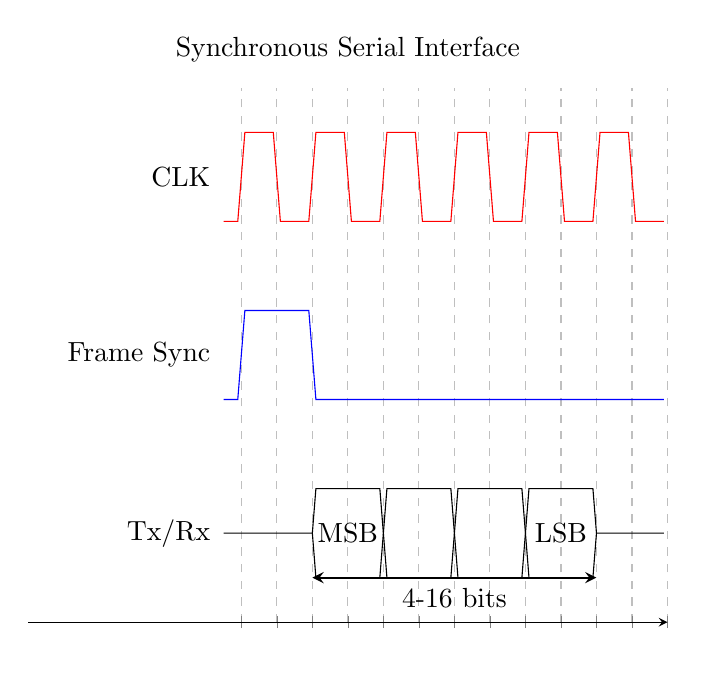
\begin{tikzpicture}
        \begin{axis}[
            width=0.8\textwidth,
            axis x line=middle,
            axis y line=none,
            xmajorgrids=true,
            grid style=dashed,
            xtick={0,10,...,120},
            xmin=-60,
            xmax=120,
            samples=1200,
            title=Synchronous Serial Interface,
            xticklabels=\empty,
        ]

        \addplot[red] coordinates
        {(-5,9) (-1,9) (1,11) (9,11) (11,9) (19,9) (21,11) (29,11) (31,9) (39,9) (41,11) (49,11)
        (51,9) (59,9) (61,11) (69,11) (71,9) (79,9) (81,11) (89,11) (91,9) (99,9) (101,11) (109,11)
        (111,9) (119,9)};

        \node[left] at (axis cs:-6,10) {CLK};
        \node[] at (axis cs:30,2) {MSB};
        \node[] at (axis cs:90,2) {LSB};

        \addplot[blue] coordinates
        {(-5,5) (-1,5) (1,7) (19,7) (21,5) (119,5)};
        
        \node[left] at (axis cs:-6,6) {Frame Sync};

        \addplot[black] coordinates
        {(-5,2) (20,2) (21,3) (39,3) (41,1) (59,1) (61,3) (79,3) (81,1) (99,1) (100,2) (119,2)};
        \addplot[black] coordinates
        {(20,2) (21,1) (39,1) (41,3) (59,3) (61,1) (79,1) (81,3) (99,3) (100,2)};
        
        \node[left] at (axis cs:-6,2) {Tx/Rx};
        \draw[darrow] (axis cs:20,1) -- (axis cs:100,1) node[midway,below] {4-16 bits};
        \end{axis}
    \end{tikzpicture}
\end{center}
\caption{Single SSI Trasmission}
\label{fig:ssi-wave}
\end{figure}


\subsection{SPI}
Serial Peripheral Interface (SPI), uses a master-slave model, is single ended, duplex, multipoint
and uses selection line based framing.

\begin{figure}[H]
\begin{center}
    \resizebox{\textwidth}{!}{
    \begin{circuitikz}
        \ctikzset{multipoles/thickness=3}
        \ctikzset{multipoles/dipchip/width=2}

        \draw (0,0) node[dipchip, num pins=6, hide numbers, no topmark, external pins
       width=0](msr) {MSR};
        \draw (msr.bpin 2) ++(0,0.1) -- ++(0.1,-0.1) -- ++(-0.1,-0.1);
        \draw (msr.bpin 1) node[right] {\tiny D}
            (msr.bpin 2) node[right] {\tiny CLK}
            (msr.bpin 3) node[right] {\tiny LOAD}
            (msr.bpin 6) node[left] {\tiny Q};
        \draw[line width=3pt] (-3,1.5) node[left] {Tx Data Bus} -| (msr.n);
        \draw[line width=3pt] (msr.s) |- (-3,-1.5) node[left] {Rx Data Bus};

        \draw (0,-5) node[dipchip, num pins=6, hide numbers, no topmark, external pins
       width=0](mfc) {MFC};
        \draw (mfc.bpin 2) ++(0,0.1) -- ++(0.1,-0.1) -- ++(-0.1,-0.1);
        \draw (mfc.bpin 1) node[right] {\tiny CNT} 
            (mfc.bpin 2) node[right] {\tiny CLK}
            (mfc.bpin 4) node[left] {\tiny RDY}
            (mfc.bpin 5) node[left] {\tiny SCK};
        
        \draw (8,0) node[dipchip, num pins=6, hide numbers, no topmark, external pins
       width=0](ssr) {SSR};
        \draw (ssr.bpin 2) ++(0,0.1) -- ++(0.1,-0.1) -- ++(-0.1,-0.1);
        \draw (ssr.bpin 1) node[right] {\tiny D}
            (ssr.bpin 2) node[right] {\tiny CLK}
            (ssr.bpin 6) node[left] {\tiny Q}
            (ssr.bpin 4) node[left] {\tiny LOAD};
        \draw[line width=2pt] (11, 1.5) node[right] {Tx Data Bus} -| (ssr.n);
        \draw[line width=2pt] (ssr.s) |- (11,-1.5) node[right] {Rx Data Bus};

        \draw (8,-5) node[dipchip, num pins=6, hide numbers, no topmark, external pins
       width=0](sfc) {SFC};
        \draw (sfc.bpin 2) ++(0,0.1) -- ++(0.1,-0.1) -- ++(-0.1,-0.1);
        \draw (sfc.bpin 2) node[right] {\tiny CLK}
            (sfc.bpin 6) node[left] {\tiny RDY};

        % Lines
        \draw (mfc) ++(5,0) node[buffer](buf){} (mfc.bpin 5) -- (buf.in) (buf.out) -- (sfc.bpin 2)
        ++(-0.5,0) node[circ]{} |- (ssr.bpin 2);
        \draw (mfc.bpin 5) ++(0.5,0) node[circ]{} |- (-2, -3.5) |- (msr.bpin 2);

        \draw (-3, 52 |- msr.bpin 3) node[left] {Tx Write} -- (msr.bpin 3)
            ++(-1, 0) node[circ]{} |- (mfc.bpin 1);

        \draw (-3, 52 |- mfc.bpin 2) node[left] {Clock} -- (mfc.bpin 2);
        \draw (mfc.bpin 4) -| (2,-6.5) -- (-3,-6.5) node[left] {Rx Ready};

        \draw (msr.bpin 6) -- (ssr.bpin 1);
        \draw (ssr.bpin 6) -| (10, 1.25) -- (-2, 1.25) |- (msr.bpin 1);
        
        \draw (ssr.bpin 4) -- (11, 52 |- ssr.bpin 4) node[right]{Tx Write};

        \draw (sfc.bpin 6) -- (11, 52 |- sfc.bpin 6) node[right]{Rx Ready};

        \draw (0,-6) node[right]{}
            ++(0,-0,5) node[right] {SSR=Slave Shift Register}
            ++(0,-0.5) node[right] {MSR=Master Shift Register}
            ++(0,-0.5) node[right] {MFC=Master Frame Counter}
            ++(0,-0.5) node[right] {SFC=Slave Frame Counter}
            ++(0,-0.5) node[right] {MOSI=Master out Slave in}
            ++(0,-0.5) node[right] {MISO=Master in Slave out}
            ++(0,-0.5) node[right] {SCK=Serial Clock};
    \end{circuitikz}
}
\end{center}
\caption{Circuit Diagram for SPI}
\label{fig:spi}
\end{figure}

SPI can be considered a simplified version of SSI, without frame synchronisation. The waveform for
the SPI protocol is shown in Figure \ref{fig:spi-wave}

\subsection{UART}
Universal Asynchronous Receive Transmit (UART) is a simple full duplex asynchronous serial
interface. UART has not framing beyond a single byte and required matched settings at both the
receiver and transmitter to avoid incorrect communications. UART has relatively high overheads and
can operate at most at 80\% efficiency. UART is also a free form protocol so can be adapted in
software to suit the application.

\begin{figure}[H]
\begin{center}
    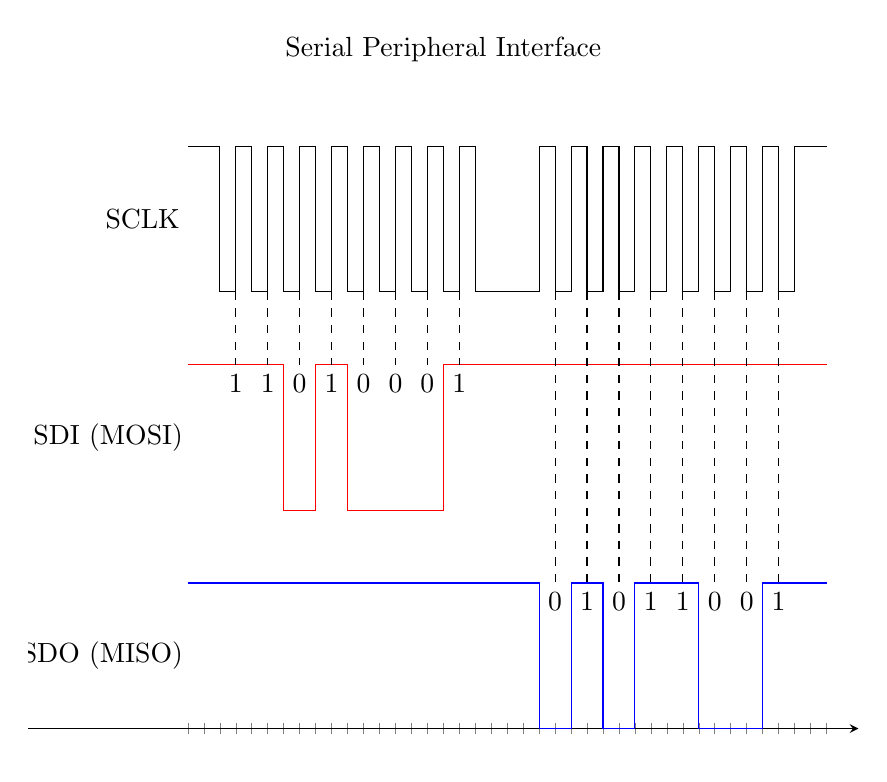
\begin{tikzpicture}
    \begin{axis}[
        width=\textwidth,
        axis x line=middle,
        axis y line=none,
        xmajorgrids=false,
        grid style=dashed,
        xtick={0,10,...,400},
        xmin=-100,
        xmax=420,
        samples=1000,
        title=Serial Peripheral Interface,
        xticklabels=\empty,
    ]
    % SCK
    \addplot[black] coordinates
    {(0,8) (20,8) (20,6) (30,6) (30,8) (40,8) (40,6) (50,6) (50,8) (60,8) (60,6) (70,6) (70,8)
    (80,8) (80,6) (90,6) (90,8) (100,8) (100,6) (110,6) (110,8) (120,8) (120,6) (130,6) (130,8) 
    (140,8) (140,6) (150,6) (150,8) (160,8) (160,6) (170,6) (170,8) (180,8) (180,6) (220,6) 
    (220,8) (230,8) (230,6) (240,6) (240,8) (250,8) (250,6) (260,6) (260,8) (270,8) (270,6)
    (280,6) (280,8) (290,8) (290,6) (300,6) (300,8) (310,8) (310,6) (320,6) (320,8) (330,8) (330,6) 
    (340,6) (340,8) (350,8) (350,6) (360,6) (360,8) (370,8) (370,6) (380,6) (380,8) (400,8)};
    
    % SDI (MOSI)
    \addplot[red] coordinates
    {(0,5) (60,5) (60,3) (80,3) (80,5) (100,5) (100,3) (160,3) (160,5) (400,5)};
    
    % SDO (MISO)
    \addplot[blue] coordinates
    {(0,2) (220,2) (220,0) (240,0) (240,2) (260,2) (260,0) (280,0) (280,2) (320,2) (320,0) (360,0)
    (360,2) (400,2)};

    % Draw Dashed Lines
    \draw[dashed] (axis cs:30,6) -- (axis cs:30,5) node[below] {1}
        (axis cs:50,6) -- (axis cs:50,5) node[below] {1}
        (axis cs:70,6) -- (axis cs:70,5) node[below] {0}
        (axis cs:90,6) -- (axis cs:90,5) node[below] {1}
        (axis cs:110,6) -- (axis cs:110,5) node[below] {0}
        (axis cs:130,6) -- (axis cs:130,5) node[below] {0}
        (axis cs:150,6) -- (axis cs:150,5) node[below] {0}
        (axis cs:170,6) -- (axis cs:170,5) node[below] {1};

    \draw[dashed] (axis cs:230,6) -- (axis cs:230,2) node[below] {0}
    (axis cs:250,6) -- (axis cs:250,2) node[below] {1}
    (axis cs:270,6) -- (axis cs:270,2) node[below] {0}
    (axis cs:290,6) -- (axis cs:290,2) node[below] {1}
    (axis cs:310,6) -- (axis cs:310,2) node[below] {1}
    (axis cs:330,6) -- (axis cs:330,2) node[below] {0}
    (axis cs:350,6) -- (axis cs:350,2) node[below] {0}
    (axis cs:370,6) -- (axis cs:370,2) node[below] {1};

    % Draw SDI, SCK etc.
    \draw (axis cs:1,7) node[left] {SCLK}
        (axis cs:3,4) node[left] {SDI (MOSI)}
        (axis cs:3,1) node[left] {SDO (MISO)};

    \end{axis}
    \end{tikzpicture}
\end{center}
\caption{SPI Transmission Waveform}
\label{fig:spi-wave}
\end{figure}


\subsection{I$^2$C/TWI}
Inter-integrated circuit (I$^2$C) or Two wire interface (TWI) is a simple, robust a d easy to use
communication system for use between a microcontroller and several external peripherals (bus type
protocol). I$^2$C is availible in standard speed at 100kbps, full-speed at 400kbps and high-speed
at 3.33Mbps. The bus supports up to 127 devices in parallel. The protocol is half duplex and
synchronous (\textit{More complicated than SPI with slave select}). This protocol is robust as every
byte has an ACK response to verify the receipt of the message, there is also built in arbitration to
eliminate bus conflicts using Carrier sense multiple access/collision detection.\\

\noindent The protocol uses 8-bit words and master slave handshaking where the master generates the clock
signal and initiates the communication. Within the transmission there is an address byte for device
selection, a read write bit for declaring reading and writing operations.\\

\subsubsection{Clock Stretching}
Clock stretching is when a slow slave device pulls the clock line low until it is ready to transmit
data, this allows the slower device to send at a usable rate for its application.

\begin{figure}[H]
\begin{center}
    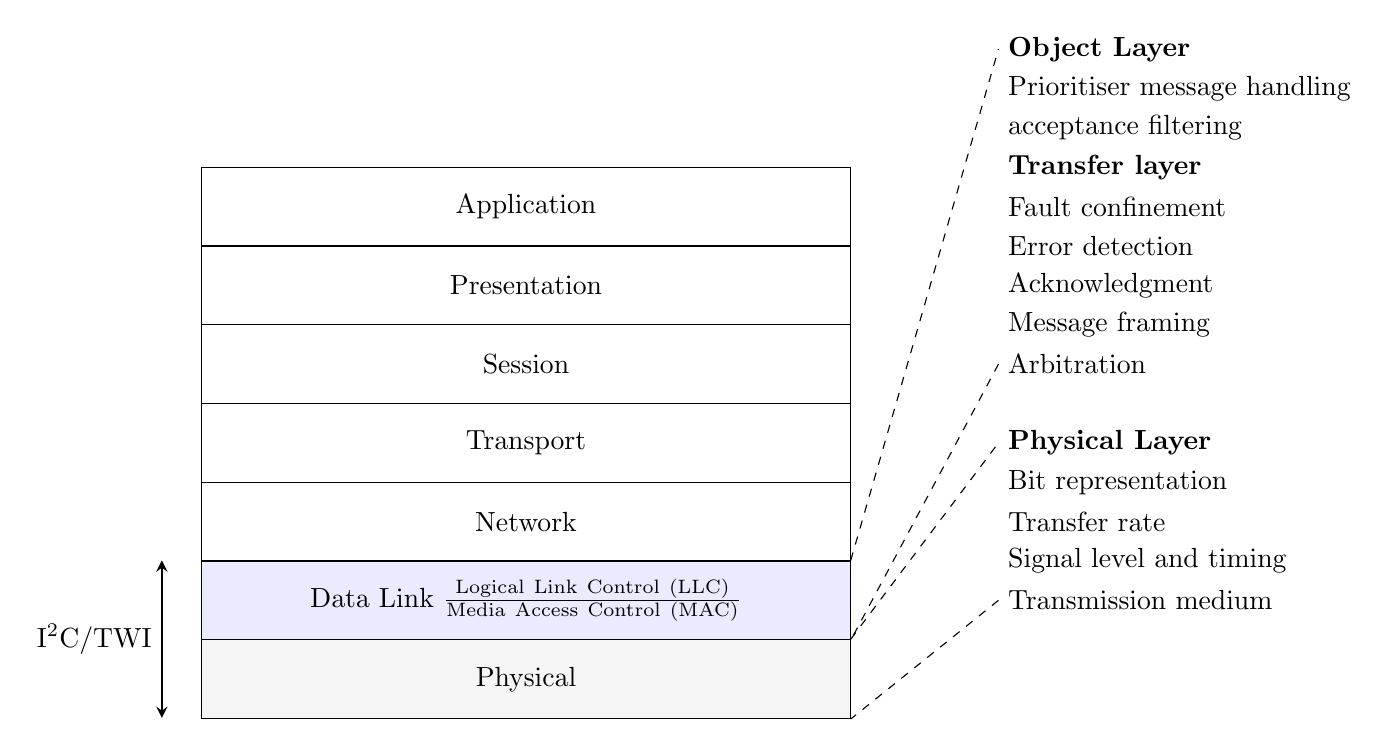
\begin{tikzpicture}
        \node[xwboxes] (app) {Application};
        \node[xwboxes, below of=app] (pres) {Presentation};
        \node[xwboxes, below of=pres] (sess) {Session};
        \node[xwboxes, below of=sess] (tran) {Transport};
        \node[xwboxes, below of=tran] (net) {Network};
        \node[xwboxes, below of=net, fill=blue!8] (data) {Data Link $\frac{\textrm{Logical Link
        Control (LLC)}}{\textrm{Media Access Control (MAC)}}$};
        \node[xwboxes, below of=data, fill=gray!8] (phy) {Physical};

        % Label
        \draw[darrow] (data.north west) ++(-0.5,0)  -- ++(0,-2) node[left, midway] {I$^2$C/TWI};

        % Info
        \draw[dashed] (data.north east) -- (6, 2) node[right]{\textbf{Object Layer}}
            ++(0, -0.5) node[right] {Prioritiser message handling}
            ++(0,-0.5) node[right] {acceptance filtering}
            ++(0, -0.5) node[right] {\textbf{Transfer layer}}
            ++(0,-0.5) node[right] {Fault confinement}
            ++(0,-0.5) node[right] {Error detection}
            ++(0,-0.5) node[right] {Acknowledgment}
            ++(0,-0.5) node[right] {Message framing}
            ++(0,-0.5) node[right] {Arbitration} -- (data.south east);

        \draw[dashed] (phy.north east) -- (6,-3) node[right] {\textbf{Physical Layer}}
           ++(0,-0.5) node[right] {Bit representation} 
           ++(0,-0.5) node[right] {Transfer rate} 
           ++(0,-0.5) node[right] {Signal level and timing} 
           ++(0,-0.5) node[right] {Transmission medium} -- (phy.south east); 
    \end{tikzpicture}
\end{center}
\caption{OSI Protocol stack for I$^2$C/TWI}
\label{fig:i2c-osi}
\end{figure}


The process of a master to slave transmission is shown in Figure \ref{fig:i2c-master-slave}.

\begin{figure}[H]
\begin{center}
\begin{adjustbox} {height=0.9\textheight}
    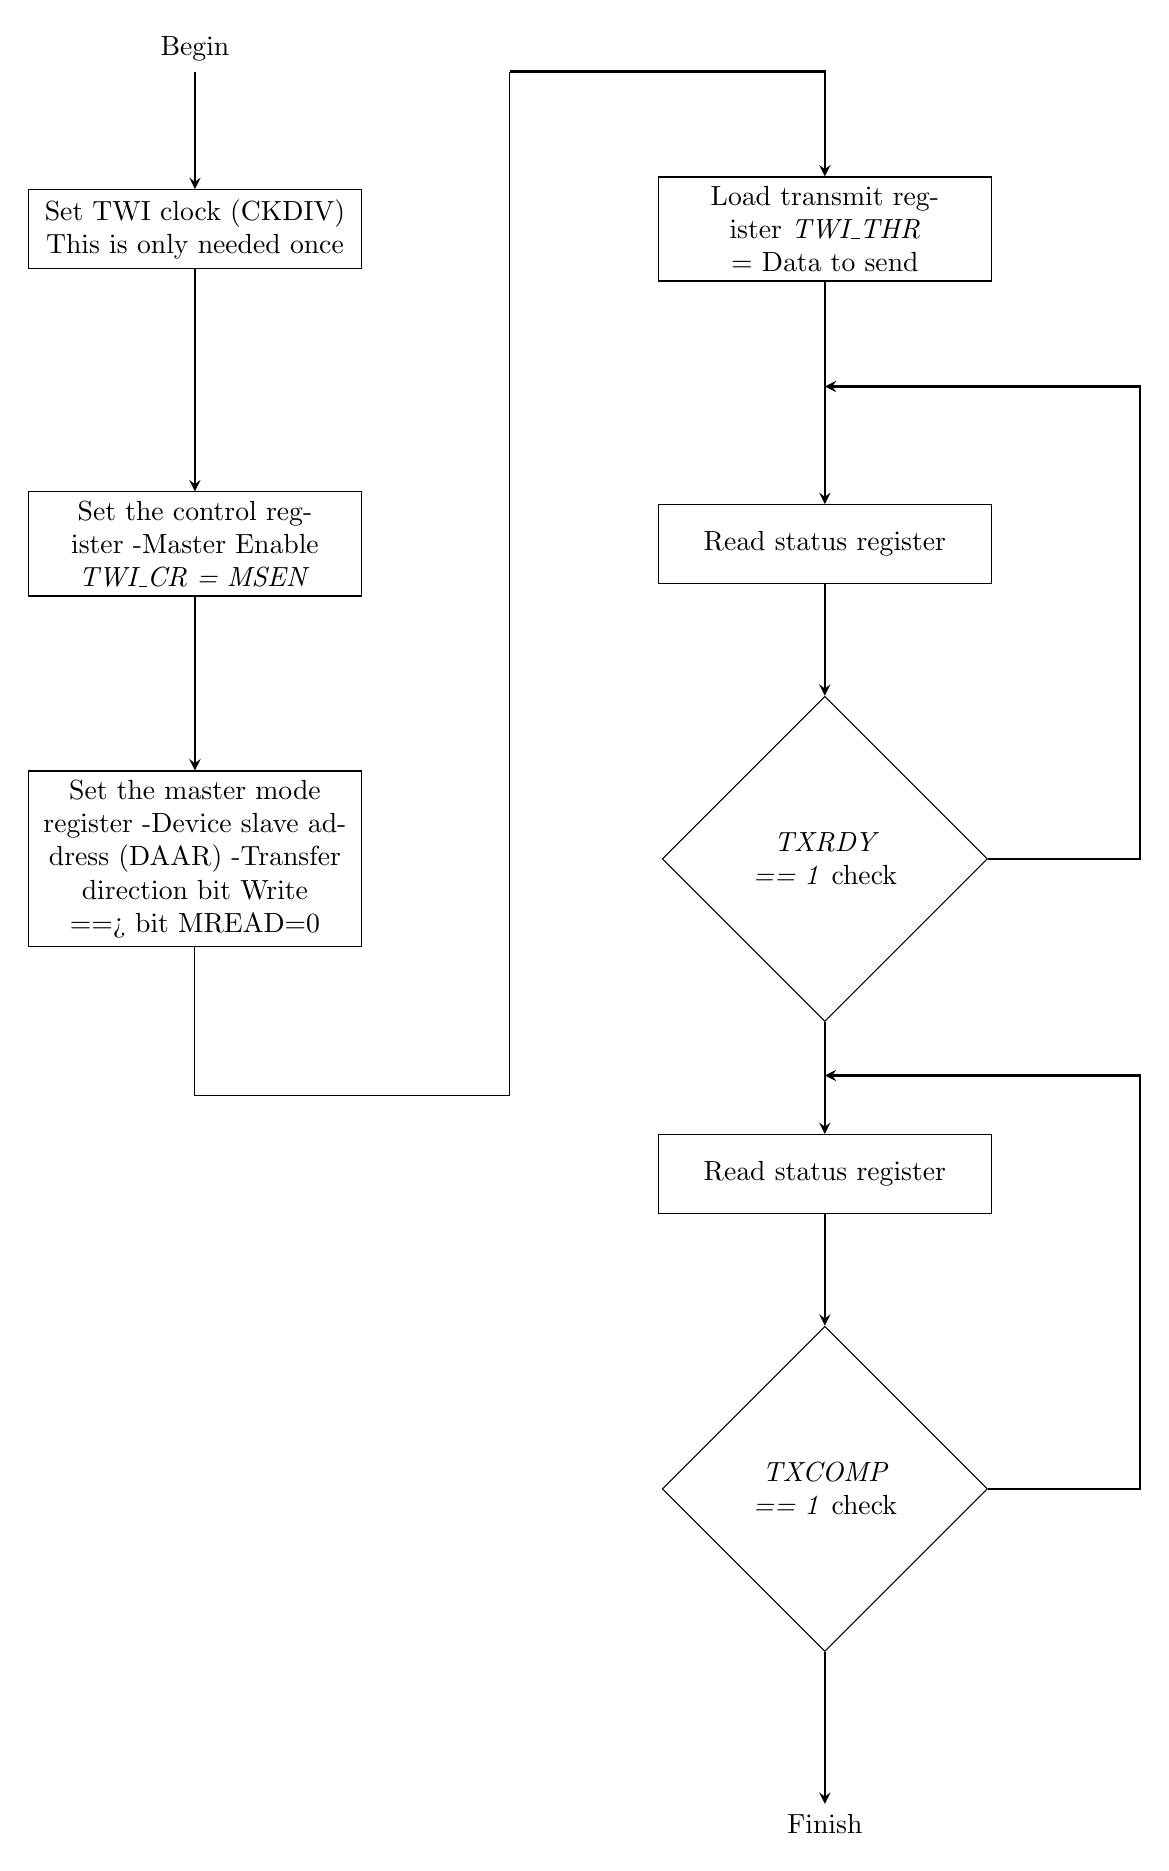
\begin{tikzpicture}
        \draw (0,0) node[wwboxes] (0) {Set TWI clock (CKDIV) This is only needed once};
        \draw (0,-4) node[wwboxes] (1) {Set the control register -Master Enable \textit{TWI\_CR = MSEN}};
        \draw (0,-8) node[wwboxes] (2) {Set the master mode register -Device slave address (DAAR)
        -Transfer direction bit Write ==> bit MREAD=0};
        \draw (8,0) node[wwboxes] (3) {Load transmit register \textit{TWI\_THR} = Data to send};
        \draw (8,-4) node[wwboxes] (4) {Read status register};
        \draw (8,-8) node[wdiamond] (5) {\textit{TXRDY == 1} check};
        \draw (8,-12) node[wwboxes] (6) {Read status register};
        \draw (8,-16) node[wdiamond] (7) {\textit{TXCOMP == 1} check};
        
        % Draw Arrows
        \draw[arrow] (0,2) node[above] {Begin} -- (0.north);
        \draw[arrow] (0.south) -- (1.north);
        \draw[arrow] (1.south) -- (2.north);
        \draw (2.south) |- (4,-11);
        \draw (4,-11) -- (4,2);
        \draw[arrow] (4,2) -| (3.north);
        \draw[arrow] (3.south) -- (4.north);
        \draw[arrow] (4.south) -- (5.north);
        \draw[arrow] (5.south) -- (6.north);
        \draw[arrow] (6.south) -- (7.north);
        \draw[arrow] (7.south) -- (8,-20) node[below] {Finish};

        \draw[arrow] (5.east) -- (12,-8) |- (8,-2);
        \draw[arrow] (7.east) -- (12,-16) |- (8,-10.75);
    \end{tikzpicture}
\end{adjustbox}
\end{center}
\caption{Master to slave transfer process and signaling on I$^2$C}
\label{fig:i2c-master-slave}
\end{figure}


\subsubsection{I$^2$C Write}
To write to a slave the send the start condition and starts the clock then send the 7-bit slave
address with the MSB first. The master then send the `0' write bit the slave then responds with an
ACK (`0'). The master then sends data (This can be several bytes). The slave then sends an ACK (`0')
and finally the master sends the stop condition.

\subsubsection{I$^2$C Read}
To read from a slave the master sends the start condition then starts the clock. The 7-bit slave
address is then transmitted with MSB first. To indicate a read the master then sends a `1' read bit.
The selected slave then responds with a ACK (`0'). The slave then sends the appropriate bit stream
(This can be several bytes). The master finally responds with a NACK then the stop condition.\\ 

\noindent To complete a full read from an external sensor the master must frist perform a write
operation to the slave then perform a read.

\subsubsection{Packet Structure}
The packet structure of I$^2$C is shown in Figure \ref{fig:serial-packet}, This is for writing, to
preform a read operation the R/W bit is set to `1' to indicate a read and in the data byte a NACK is
used instead of the ACK (\textit{ACK=1, NACK=0}). 
\begin{figure}[H]
\begin{center}
    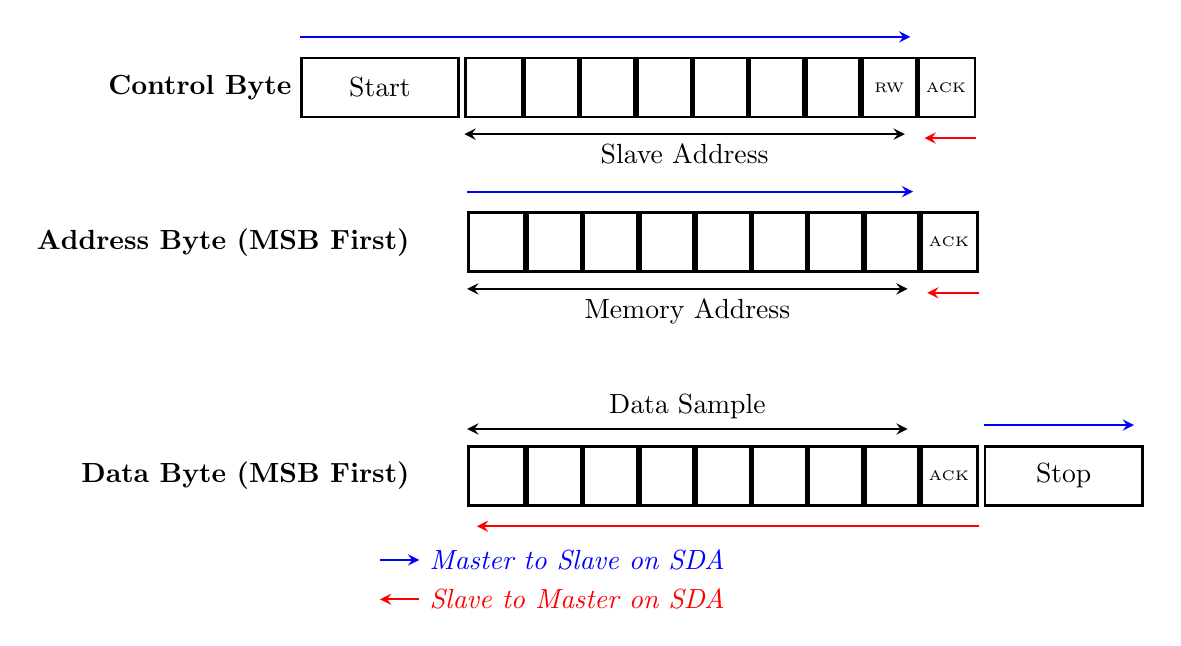
\begin{tikzpicture}
        \node[smboxes] (start) {Start};
        \node[xsmboxes, right of=start, xshift=1.5cm] (0) {};
        \node[xsmboxes, right of=0, xshift=0.75cm] (1) {};
        \node[xsmboxes, right of=1, xshift=0.75cm] (2) {};
        \node[xsmboxes, right of=2, xshift=0.75cm] (3) {};
        \node[xsmboxes, right of=3, xshift=0.75cm] (4) {};
        \node[xsmboxes, right of=4, xshift=0.75cm] (5) {};
        \node[xsmboxes, right of=5, xshift=0.75cm] (6) {};
        \node[xsmboxes, right of=6, xshift=0.75cm] (7) {\tiny RW};
        \node[xsmboxes, right of=7, xshift=0.75cm] (ACK) {\tiny ACK};
       
        
        \node[xsmboxes, below of=start, yshift=-2cm, xshift=1.5cm] (01) {};
        \node[xsmboxes, right of=01, xshift=0.75cm] (11) {};
        \node[xsmboxes, right of=11, xshift=0.75cm] (21) {};
        \node[xsmboxes, right of=21, xshift=0.75cm] (31) {};
        \node[xsmboxes, right of=31, xshift=0.75cm] (41) {};
        \node[xsmboxes, right of=41, xshift=0.75cm] (51) {};
        \node[xsmboxes, right of=51, xshift=0.75cm] (61) {};
        \node[xsmboxes, right of=61, xshift=0.75cm] (71) {};
        \node[xsmboxes, right of=71, xshift=0.75cm] (ACK1) {\tiny ACK};
        
        \node[xsmboxes, below of=01, yshift=-3cm] (02) {};
        \node[xsmboxes, right of=02, xshift=0.75cm] (12) {};
        \node[xsmboxes, right of=12, xshift=0.75cm] (22) {};
        \node[xsmboxes, right of=22, xshift=0.75cm] (32) {};
        \node[xsmboxes, right of=32, xshift=0.75cm] (42) {};
        \node[xsmboxes, right of=42, xshift=0.75cm] (52) {};
        \node[xsmboxes, right of=52, xshift=0.75cm] (62) {};
        \node[xsmboxes, right of=62, xshift=0.75cm] (72) {};
        \node[xsmboxes, right of=72, xshift=0.75cm] (ACK2) {\tiny ACK};
        \node[smboxes, right of=ACK2, xshift=1.5cm] (stop) {Stop};

        \draw (7.north east) ++(0,0.25) node[] (controlend) {};
        \draw (ACK.south west) ++(0,-0.25) node[] (ACKstart) {};
        \draw (71.north east) ++(0,0.25) node[] (addrend) {};
        \draw (ACK1.south west) ++(0,-0.25) node[] (ACK1start) {};
        \draw (02.south west) ++(0,-0.25) node[] (datastart) {};
        \draw (stop.north east) ++(0,0.25) node[] (stopend) {};
        \draw (ACK.south west) ++(0,-0.2) node[] (ACKstartlabel) {};
        \draw (ACK1.south west) ++(0,-0.2) node[] (ACK1startlabel) {};
        \draw (ACK2.north west) ++(0,0.2) node[] (ACK2startlabel) {};

        % Arrows
        \draw[arrow, blue] (start.north west) ++(0,0.25) -- (controlend);
        \draw[arrow, red] (ACK.south east) ++(0,-0.25) -- (ACKstart);
        \draw[arrow, blue] (01.north west) ++(0,0.25) -- (addrend);
        \draw[arrow, red] (ACK1.south east) ++(0,-0.25) -- (ACK1start);
        \draw[arrow, blue] (stop.north west) ++(0,0.25) -- (stopend);
        \draw[arrow, red] (ACK2.south east) ++(0,-0.25) -- (datastart);

        % Text Labels
        \draw (start) ++(-1,0) node[left] {\textbf{Control Byte}};
        \draw (01) ++(-1,0) node[left] {\textbf{Address Byte (MSB First)}};
        \draw (02) ++(-1,0) node[left] {\textbf{Data Byte (MSB First)}};

        % Byte Labels
        \draw[darrow] (0.south west) ++(0,-0.2) -- (ACKstartlabel) node[below,midway] {Slave Address};
        \draw[darrow] (01.south west) ++(0,-0.2) -- (ACK1startlabel) node[below,midway] {Memory
        Address};
        \draw[darrow] (02.north west) ++(0,0.2) -- (ACK2startlabel) node[above,midway] {Data
        Sample};

        % Key
        \draw[arrow,blue] (0,-6) -- ++(0.5, 0) node[right] {\textit{Master to Slave on SDA}};
        \draw[arrow,red] (0.5,-6.5) node[right] {\textit{Slave to Master on SDA}} -- ++(-0.5,0);

    \end{tikzpicture}
\end{center}
\caption{Serial Packet Structure}
\label{fig:serial-packet}
\end{figure}


\subsubsection{Multi-master Operation}
Multi-master operation is supported on I$^2$C however, in this mode arbitration is required as
several masters may attempt to control the bus simultaneously. For this to work every master in a
multi-master must be configured to a multi-master setup as single masters don't arbitrate, causing
interference if a single master is connected. The master device controls SDA and SCK.

Arbitration simply allows the faster (or slower) device to access the channel. To detect if the
channel is in use the SDA and SCL lines are checked to see if they are LOW.

\subsubsection{Collision Detection}
A collision is where more than one device is transmitting on the SDA line at once. To perform
collision detection a device has to be able to read the SDA line while checking the SDA for
transmitted bits. And if the two don't match then a collision has occurred. This is determined using
the XOR of the requested bit and the line data, shown in Figure \ref{fig:collision-detect}.

\begin{figure}[H]
\begin{center}
    \begin{circuitikz}[american]
        \node[xor port, rotate=-90] at (2, -2) (xor) {};
        \node[pmos] at (5, -1.25) (fet){};

        % Draw Lines
        \draw (0,0) -| (fet.source);
        \draw (0,0) -- (6,0) node[right] {SDA};
        \draw (fet.drain) -- ++(0,-0.5) node[ground]{};

        \draw (0,-0.5) -| (fet.gate);
        \draw(0,-0.5) -| (xor.in 2);
        \draw (0,0) -| (xor.in 1);
        \draw (xor.out) |- (0,-3) node[left] {Collision};

        \node[left] at (0,0) {RXD};
        \node[left] at (0,-0.5) {TXD};
    \end{circuitikz}
\end{center}
\caption{I$^2$C Collision Detection Circuitry}
\label{fig:collision-detect}
\end{figure}



\section{CAN}
Control Area Network (CAN) is a noise resilient, asynchronous half-duplex serial protocol. The
protocol uses a broadcast bus topology with no specific device/chip address. CAN also has message
identifiers and message priority as well as type. Messages can also be processed by multiple nodes
(\textit{functional addressing})\\

\noindent The two wire structure supports 1Mbps for distances 40m, 120kbps possible over 500m and 
5kbps over 10km. CAN-FD (\textit{flexible data rate}) increased the speed by a factor of 5.\\

\noindent CAN uses multi-master/controller system with carrier sense multiple access with collision
detection (CSMA/CD). CAN also uses arbitration on message priority (AMP), this is a non-destructive
form of arbitration with is important for hard deadline, real-time and distributed systems. The
priority order is the lower the number the higher the priority ie. 0 is the highest priority.\\

\noindent CAN uses non-return to zero (NRZ) line coding this causes difficulty in clock
synchronisation for long strings of `1' and `0'. This means that CAN requires falling or rising
edges for every 5 bits, so after five bits of the same level, a 6\textsuperscript{th} inverse bit is
added to the transmission. These bits are then removed at the receivers.

\begin{figure}[H]
\begin{center}
    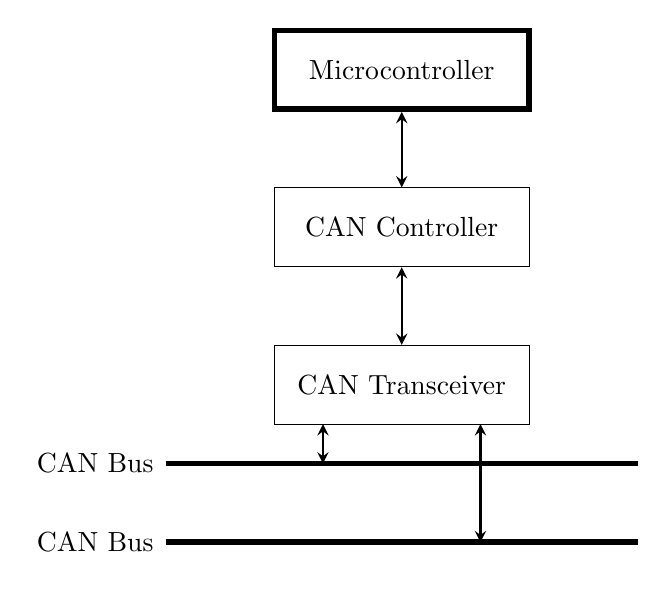
\begin{tikzpicture}
        \node[wboxes, line width=2pt] (micro) {Microcontroller};
        \node[wboxes, below of=micro, yshift=-1cm] (control) {CAN Controller};
        \node[wboxes, below of=control, yshift=-1cm] (tran){CAN Transceiver};

        \draw[line width=2pt] (-3,-5) node[left] {CAN Bus} -- (3,-5);
        \draw[line width=2pt] (-3,-6) node[left] {CAN Bus} -- (3,-6);
        \draw[darrow] (-1,-5) -- (-1,-4.5);
        \draw[darrow] (1,-6) -- (1,-4.5);
        \draw[darrow] (tran) -- (control);
        \draw[darrow] (control) -- (micro);

    \end{tikzpicture}
\end{center}
\caption{CAN Block Diagram}
\label{fig:can=block}
\end{figure}

\noindent The two wires used in CAN are a differential pair, this increases noise resilience which
is important in the automotive sector where this protocol was designed. This bus also still works if
the bus is broken of shorted to either power or ground. To represent a `1' bit the pair is
\textit{recessive}, this is where $\textrm{CAN}_H \approx \textrm{CAN}_L \approx V_{cc}/2$ to
represent a `0' bit the pair is \textit{dominant} this is where $\textrm{CAN}_H > \textrm{CAN}_L$
this behaviour is shown in Figure \ref{fig:can-wave}.

\begin{figure}[H]
\begin{center}
    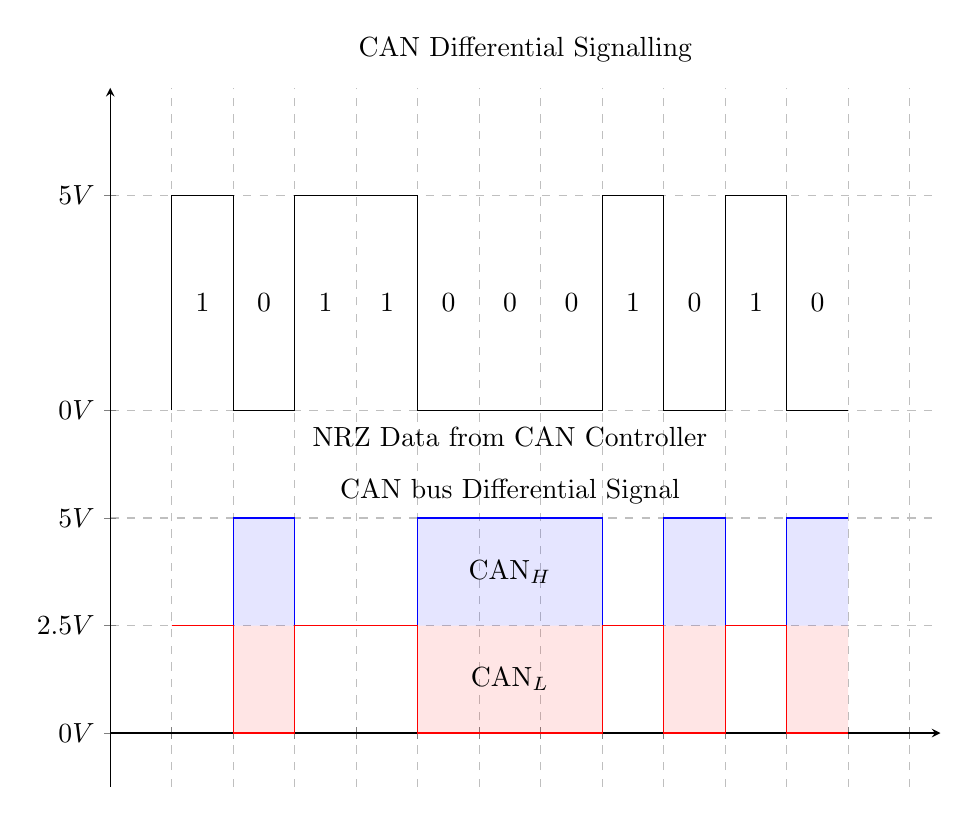
\begin{tikzpicture}
    \begin{axis}[
        width=\textwidth,
        axis x line=middle,
        axis y line=left,
        xmajorgrids=true,
        ymajorgrids=true,
        grid style=dashed,
        xtick={0,10,...,120},
        ytick={\empty},
        extra y ticks={0,1,2,3,5},
        extra y tick labels={$0V$, $2.5V$, $5V$, $0V$, $5V$},
        xmin=-10,
        xmax=125,
        ymin=-0.5,
        ymax=6,
        samples=1000,
        title=CAN Differential Signalling,
        xticklabels=\empty,
    ]

    \addplot[black] coordinates
    {(0,3) (0,5) (10,5) (10,3) (20,3) (20,5) (40,5) (40,3) (70,3) (70,5) (80,5) (80,3) (90,3) (90,5)
    (100,5) (100,3) (110,3)};

    \addplot[blue, name path=canh] coordinates
    {(0,1) (10,1) (10,2) (20,2) (20,1) (40,1) (40,2) (70,2) (70,1) (80,1) (80,2) (90,2) (90,1)
    (100,1) (100,2) (110,2)};

    \addplot[red, name path=canl] coordinates
    {(0,1) (10,1) (10,0) (20,0) (20,1) (40,1) (40,0) (70,0) (70,1) (80,1) (80,0) (90,0) (90,1)
    (100,1) (100,0) (110,0)};

    \path[name path=middle] (axis cs:0,1) -- (axis cs:110,1);
    \addplot[
        color=red,
        fill=red,
        fill opacity=0.1,
    ] fill between[
        of=middle and canl,
        soft clip={domain=0:110},
    ];
    
    \addplot[
        color=blue,
        fill=blue,
        fill opacity=0.1,
    ] fill between[
        of=middle and canh,
        soft clip={domain=0:110},
    ];

    % Draw Bits
    \draw (axis cs:5,4) node[] {1}
        (axis cs:15,4) node[] {0}
        (axis cs:25,4) node[] {1}
        (axis cs:35,4) node[] {1}
        (axis cs:45,4) node[] {0}
        (axis cs:55,4) node[] {0}
        (axis cs:65,4) node[] {0}
        (axis cs:75,4) node[] {1}
        (axis cs:85,4) node[] {0}
        (axis cs:95,4) node[] {1}
        (axis cs:105,4) node[] {0};
    

    % Draw Labels
    \draw (axis cs:55,1.5) node[] {CAN$_H$};
    \draw (axis cs:55,0.5) node[] {CAN$_L$};
    \draw (axis cs:55,2.75) node[] {NRZ Data from CAN Controller};
    \draw (axis cs:55,2.25) node[] {CAN bus Differential Signal};
    
    \end{axis}
    \end{tikzpicture}
\end{center}
\caption{CAN Differential Signalling}
\label{fig:can-wave}
\end{figure}


The idle state of CSMA CAN is recessive (`1'). To avoid collisions CAN monitors bit transmissions.

\subsection{CAN Message Format}
The following figure describes the packet format of a CAN message.

\begin{figure}[H]
\begin{center}
    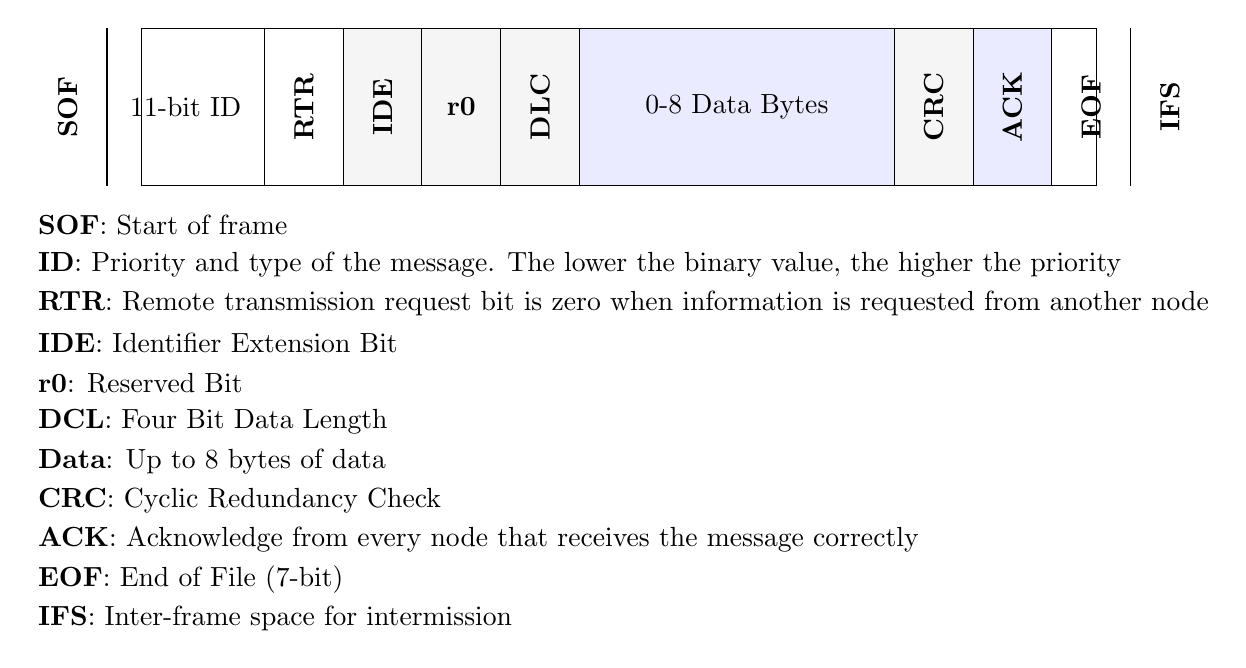
\begin{tikzpicture}
        \node[boxes, minimum height=2cm, minimum width=\textwidth] at (7.5,0) (box) {};

        % Fill the boxes first to stop overlaying text
        \draw[fill=gray, fill opacity=0.08] (4,1) -- (5,1) -- (5,-1) -- (4,-1) -- (4,1);
        \draw[fill=gray, fill opacity=0.08] (5,1) -- (6,1) -- (6,-1) -- (5,-1) -- (5,1);
        \draw[fill=gray, fill opacity=0.08] (6,1) -- (7,1) -- (7,-1) -- (6,-1) -- (6,1);
        \draw[fill=blue, fill opacity=0.08] (7,1) -- (11,1) -- (11,-1) -- (7,-1) -- (7,1);
        \draw[fill=gray, fill opacity=0.08] (11,1) -- (12,1) -- (12,-1) -- (11,-1) -- (11,1);
        \draw[fill=blue, fill opacity=0.08] (12,1) -- (13,1) -- (13,-1) -- (12,-1) -- (12,1);


        \draw (1,1) -- (1,-1);
        \draw (0.5,0) node[rotate=90] {\textbf{SOF}};

        \draw (3,1) -- (3,-1);
        \draw (2,0) node[] {11-bit ID};

        \draw (4,1) -- (4,-1);
        \draw (3.5,0) node[rotate=90] {\textbf{RTR}};

        \draw (5,1) -- (5,-1);
        \draw (4.5,0) node[rotate=90] {\textbf{IDE}};

        \draw (6,1) -- (6,-1);
        \draw (5.5,0) node[] {\textbf{r0}};

        \draw (7,1) -- (7,-1);
        \draw (6.5,0) node[rotate=90] {\textbf{DLC}};

        \draw (11,1) -- (11,-1);
        \draw (9,0) node[] {0-8 Data Bytes};

        \draw (12,1) -- (12,-1);
        \draw (11.5,0) node[rotate=90] {\textbf{CRC}};

        \draw (13,1) -- (13,-1);
        \draw (12.5,0) node[rotate=90] {\textbf{ACK}};

        \draw (14,1) -- (14,-1);
        \draw (13.5,0) node[rotate=90] {\textbf{EOF}};

        \draw (14.5,0) node[rotate=90] {\textbf{IFS}};

        % Draw Key
        \draw (0,-1.5) node[right] {\textbf{SOF}: Start of frame}
            ++(0,-0.5) node[right] {\textbf{ID}: Priority and type of the message. The lower the
            binary value, the higher the priority}

            ++(0,-0.5) node[right] {\textbf{RTR}: Remote transmission request bit is zero when
            information is requested from another node}

            ++(0,-0.5) node[right] {\textbf{IDE}: Identifier Extension Bit}
            ++(0,-0.5) node[right] {\textbf{r0}: Reserved Bit}
            ++(0,-0.5) node[right] {\textbf{DCL}: Four Bit Data Length}
            ++(0,-0.5) node[right] {\textbf{Data}: Up to 8 bytes of data}
            ++(0,-0.5) node[right] {\textbf{CRC}: Cyclic Redundancy Check}
            ++(0,-0.5) node[right] {\textbf{ACK}: Acknowledge from every node that receives the
            message correctly}

            ++(0,-0.5) node[right] {\textbf{EOF}: End of File (7-bit)}
            ++(0,-0.5) node[right] {\textbf{IFS}: Inter-frame space for intermission};
    \end{tikzpicture}
\end{center}
\caption{CAN Packet Format}
\label{fig:can-packet}
\end{figure}


\subsection{CRC}
\paragraph{Parity Checks} Parity checks can be used to verify a transmission, using a \textbf{single
bit} XOR gates are used to determine the value of the parity bit. Essentially a parity bit of `1'
means that there is an odd number of `1' bits and `0' means that there is an even number of `1' bits.

\noindent The method of a parity check is given by (\ref{eqn:parity}) where the bit sequence $x$ is
`0010 0101'

\begin{equation}
\begin{aligned}
    x &= 00100101\\
    \textrm{CRC} &= x_7 \oplus x_6 \oplus x_5 \oplus x_4 \oplus x_3 \oplus x_2 \oplus x_1 \oplus
    x_0\\
    &=0 \oplus 0 \oplus 1 \oplus 0 \oplus 0 \oplus 1 \oplus 0 \oplus 1\\
    \textrm{CRC} &= 1
\end{aligned}
\label{eqn:parity}
\end{equation}

\subsubsection{CRC}
Cyclic Redundancy Check (CRC) is a $n$-bit checksum method which detects data inconsistency using
polynomial division. This uses a \textit{Dividend} which is the input data, and \textit{Divisor}
which is a given bit sequence also known as a \textit{generator polynomial} which is defined as
(\ref{eqn:generator}). The predefined generator polynomial contains $n+1$ bits.

\begin{equation}
    G=\sum_{k=0}^{k=n+1} x^k
    \label{eqn:generator}
\end{equation}

To preform a CRC:

\begin{enumerate}
\item Append the input with $n$ `0'
\item Align the 1\textsuperscript{st} `1' of the divisor with the 1\textsuperscript{st} `1' of the
dividend
\item Stop when the divisor zeros out each bit of input data
\item Return the last $n$ bits of the remainder
\end{enumerate}

A CRC-3 (3-bit CRC) check example is shown in (\ref{eqn:crc}) this shows the process of completing
the first step, with each step repeating the same way.

\begin{equation}
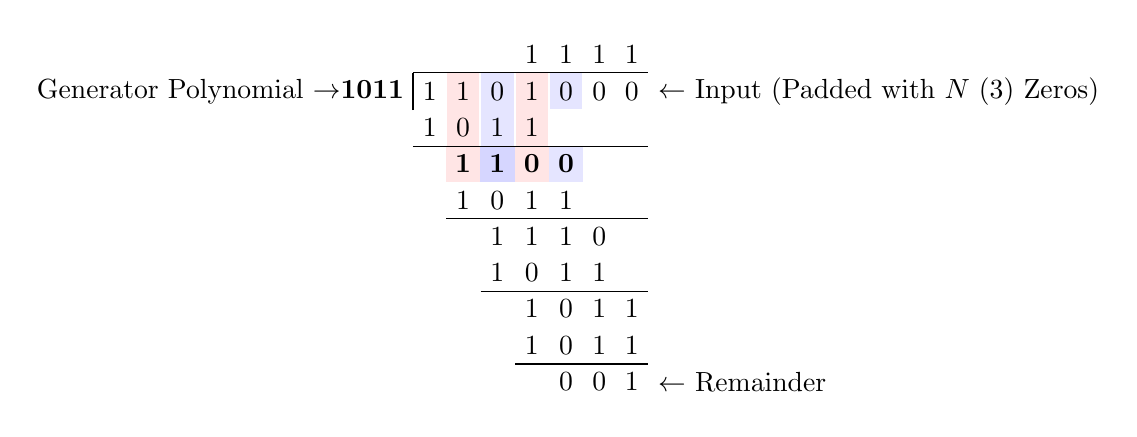
\begin{tikzpicture}[baseline={([yshift=-.5ex]current bounding box.center)}]

\node[matrix of math nodes] (div) {
    \empty & \empty & \empty & 1 & 1 & 1 & 1\\
    1 & \node[fill=red!10]{1}; & \node[fill=blue!10]{0}; & \node[fill=red!10]{1}; &
    \node[fill=blue!10]{0}; & 0 & 0\\
    1 & \node[fill=red!10]{0}; & \node[fill=blue!10]{1}; & \node[fill=red!10]{1};\\
    \empty & \node[fill=red!10]{\textbf{1}}; & \node[fill=blue!16]{\textbf{1}}; &
    \node[fill=red!10]{\textbf{0}}; & \node[fill=blue!10]{\textbf{0}};\\
    \empty & 1 & 0 & 1 & 1\\
    \empty & \empty & 1 & 1 & 1 & 0\\
    \empty & \empty & 1 & 0 & 1 & 1\\
    \empty & \empty & \empty & 1 & 0 & 1 & 1\\
    \empty & \empty & \empty & 1 & 0 & 1 & 1\\
    \empty & \empty & \empty & \empty & 0 & 0 & 1\\
};

\draw (div-3-1.south west) -- (div-2-7.south east |- div-3-1.south); 
\draw (div-5-2.south west) -- (div-2-7.south east |- div-5-2.south); 
\draw (div-7-3.south west) -- (div-2-7.south east |- div-7-3.south); 
\draw (div-9-4.south west) -- (div-2-7.south east |- div-9-4.south); 

\draw (div-2-7.east) node[right] {$\gets$ Input (Padded with $N$ (3) Zeros)};
\draw (div-10-7.east) node[right] {$\gets$ Remainder};

\draw (div-2-1) node[left, xshift=-0.2cm] {Generator Polynomial $\to$\textbf{1011}};
\draw (div-2-1.north west) -- (div-2-7.north east);
\draw (div-2-1.south west) -- (div-2-1.north west);
\end{tikzpicture}
\label{eqn:crc}
\end{equation}


\textbf{NOTE}: CAN uses CRC-15 so the generator polynomial is 16bit long and the remainder is 15bit
long.




\section{High-Speed Data Transfer Techniques}
\subsection{Block Processing}
Block processing is where the CPU processes the data blocks already stored in memory, together
without streaming more data. This is usually done with the data in vector form, see Intel AVX
instructions and ARM Neon intrinsics. An example of block processing could be a moving average
filter (MAF). For the moving average filter once it has been applied to the input data the output
must be stored in a separate memory section. This can pose issues in moving within memory and
between memory and peripherals.

\subsection{Unbuffered Data Transfer}
Unbuffered transfer is when no buffer is implemented on the input of data, this can cause
synchronization issues as both the sender and receiver need to be aware of the when the data is
transferred. A diagram of this is shown in Figure \ref{fig:unbuffered}\\

\noindent There are two methods for implementing unbuffered transfer, the first is to use
\textit{Polling}. Polling can waste CPU cycles as the CPU will have to reguarly check if data is
available. This can be somewhat mitigated through the use of the second method, \textit{Interrupts}
this method ensures that data can be transferred once it is available however, there can be
significant overhead created due to the context switch required to service the interrupt.

\begin{figure}[H]
\begin{center}
    \begin{circuitikz}
        \ctikzset{multipoles/thickness=3}
        \ctikzset{multipoles/dipchip/width=2.5}
    
        \draw (0,0) node[dipchip, num pins=6, hide numbers, no topmark, external pins
       width=0](shift) {8-bit shift register};

        \draw (0,-3) node[dipchip, num pins=6, hide numbers, no topmark, external pins
       width=0](framecount) {3-bit frame counter};

        \draw (framecount.bpin 2) ++(0,0.1) -- ++(0.1,-0.1) -- ++(-0.1,-0.1);
        \draw (shift.bpin 2) ++(0,0.1) -- ++(0.1,-0.1) -- ++(-0.1,-0.1);

        \draw (framecount.bpin 2) ++(-1.5,0) node[not port](invert){};
        
        \draw (invert.in) -- ++(-0.5,0) node[left] {SCK};
        \draw (invert.out) -- ++(0.5,0) |- (shift.bpin 2);
        \draw (invert.out) -- (framecount.bpin 2);
        
        \draw (shift.bpin 1) -- ++(-1.5,0) node[left] {MOSI};

        \draw (shift.bpin 1) node[right] {\tiny D};
        \draw (shift.s) node[above] {\tiny Q(0:7)};
        \draw[line width=3pt] (shift.s) |- (4,-1.5) node[right] {SPIDATA};
        \draw (framecount.bpin 6) -- (framecount.bpin 6 -| 4,-1.5) node[right] {SPIRDY};
    \end{circuitikz}
\end{center}
\caption{Unbuffered Data Transfer}
\label{fig:unbuffered}
\end{figure}


\subsection{Buffered Data Transfer}
By using a buffer a block of data can be transferred once the FIFO (First in First out) buffer is
full. To indicate that the buffer is full an ISR (Interrupt Service Routine) can be used. This
reduces the overhead as interrupts are occurring less frequently than with unbuffered however, there
is a latency increase as data is held until the buffer is full. This method can also be used to
transfer data without the CPU. Figure \ref{fig:buffered} shows the general format of a buffered data
transfer.

\begin{figure}[H]
\begin{center}
    \begin{circuitikz}
        \ctikzset{multipoles/thickness=3}
        \ctikzset{multipoles/dipchip/width=2.5}
    
        \draw (0,0) node[dipchip, num pins=6, hide numbers, no topmark, external pins
       width=0](shift) {8-bit shift register};

        \draw (0,-3) node[dipchip, num pins=6, hide numbers, no topmark, external pins
       width=0](framecount) {3-bit frame counter};

        \draw (4,-2) node[dipchip, num pins=6, hide numbers, no topmark, external pins
       width=0](fifo){FIFO Buffer};

        \draw (framecount.bpin 2) ++(0,0.1) -- ++(0.1,-0.1) -- ++(-0.1,-0.1);
        \draw (shift.bpin 2) ++(0,0.1) -- ++(0.1,-0.1) -- ++(-0.1,-0.1);
        \draw (fifo.bpin 3) ++(0,0.1) -- ++(0.1,-0.1) -- ++(-0.1,-0.1);

        \draw (framecount.bpin 2) ++(-1.5,0) node[not port](invert){};
        
        \draw (invert.in) -- ++(-0.5,0) node[left] {SCK};
        \draw (invert.out) -- ++(0.5,0) |- (shift.bpin 2);
        \draw (invert.out) -- (framecount.bpin 2);
        
        \draw (shift.bpin 1) -- ++(-1.5,0) node[left] {MOSI};

        \draw (shift.bpin 1) node[right] {\tiny D};
        \draw (shift.s) node[above] {\tiny Q(0:7)};
        \draw (fifo.bpin 1) node[right] {\tiny DATA};
        \draw (fifo.bpin 6) node[left] {\tiny Q};
        \draw (fifo.bpin 4) node[left] {\tiny RDY};

        \draw[line width=3pt] (shift.s) |- (fifo.bpin 1);
        \draw[line width=3pt] (fifo.bpin 6) -- ++(1,0) node[right] {SPIDATA};
        \draw (fifo.bpin 4) -- ++(1,0) node[right] {SPIRDY};
        \draw (framecount.bpin 6) -- ++(0.25,0) |- (fifo.bpin 3);
    \end{circuitikz}
\end{center}
\caption{Buffered Data Transfer}
\label{fig:buffered}
\end{figure}


\subsection{Transfer Interfaces}
There are several method to achieve high speed CPU independent data transfer between memory sections
or between memory and peripherals these include:

\begin{itemize}
    \item Host port interface (This is a MCU to MCU interface/parallel address bus, this is rare now)
    \item Buffered Serial Port (This is a peripheral to memory transfer)
    \item Dual Port Memory (This has simultaneous read and write access)
    \item Direct Memory Access (This is a programmable and cascadeable module)
\end{itemize}

\subsubsection{Dual-Port Memory}
Dual port memory (shown in Figure \ref{fig:dual-port-mem}) allows for similtaneous read/write memory
operations, to achieve this arbitration logic is required to control memory access confilicts. The
applications for this are DSP active filters and shared memory systems.

\begin{figure}[H]
\begin{center}
\begin{adjustbox}{width=\textwidth}
    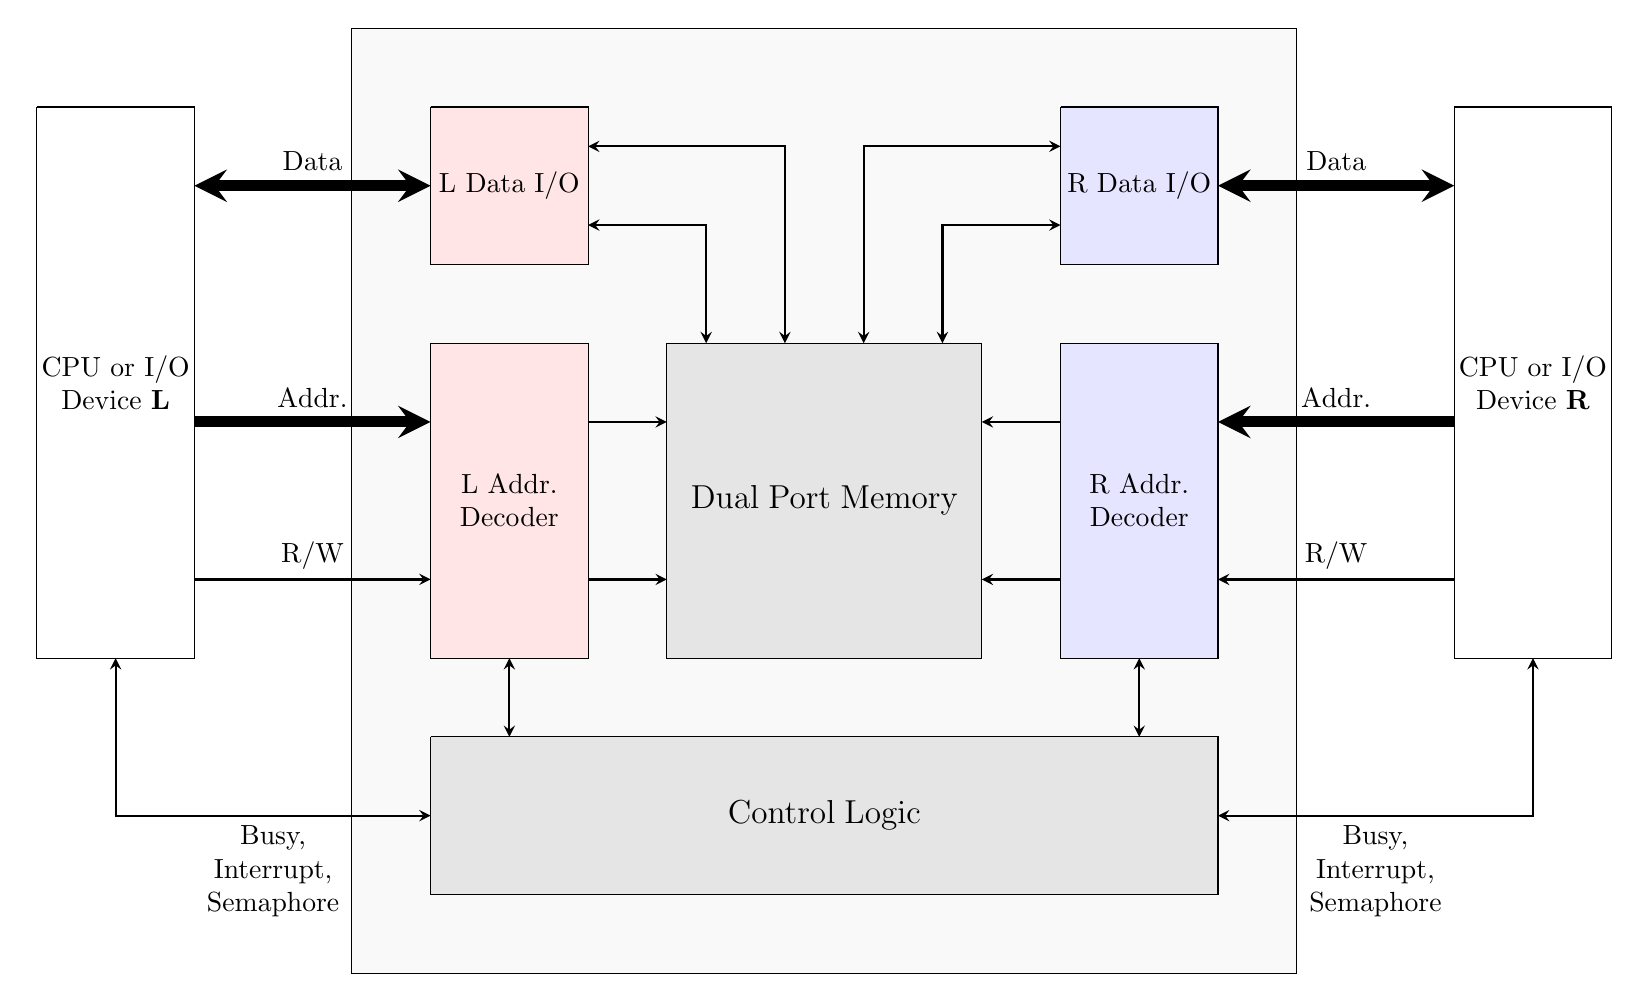
\begin{tikzpicture}
        \draw[fill=gray!5] (0,0) -- (12,0) -- (12,-12) -- (0,-12) -- (0,0);
        \draw[fill=red!10] (1,-1) -- (3,-1) -- (3,-3) -- (1,-3) -- (1,-1);
            \draw[text width=2cm, text centered]  (2,-2) node[] {L Data I/O};
        \draw[fill=blue!10] (9,-1) -- (11,-1) -- (11,-3) -- (9,-3) -- (9,-1);
            \draw[text width=2cm, text centered]  (10,-2) node[] {R Data I/O};
        \draw[fill=gray!20] (4,-4) -- (8,-4) -- (8,-8) -- (4,-8) -- (4,-4);
            \draw[text width=5cm, text centered]  (6,-6) node[] {\large Dual Port Memory};
        \draw[fill=red!10] (1,-4) -- (3,-4) -- (3,-8) -- (1,-8) -- (1,-4);
            \draw[text width=2cm, text centered] (2,-6) node[] {L Addr. Decoder};
        \draw[fill=blue!10] (9,-4) -- (11,-4) -- (11,-8) -- (9,-8) -- (9,-4);
            \draw[text width=2cm, text centered] (10,-6) node[] {R Addr. Decoder};

        \draw[fill=gray!20] (1,-9) -- (11,-9) -- (11,-11) -- (1,-11) -- (1,-9);
            \draw [text width=10cm, text centered] (6,-10) node[] {\large Control Logic};
       
        \draw (14,-1) -- (16,-1) -- (16,-8) -- (14,-8) -- (14,-1);
            \draw[text width=2cm, text centered] (15,-4.5) node[] {CPU or I/O Device \textbf{R}};

        \draw (-4,-1) -- (-2,-1) -- (-2,-8) -- (-4,-8) -- (-4,-1);
            \draw[text width=2cm, text centered] (-3,-4.5) node[] {CPU or I/O Device \textbf{L}};

        % Draw Arrows
        \draw[darrow] (2,-8) -- (2,-9);
        \draw[darrow] (10,-8) -- (10,-9);

        \draw[darrow] (3,-1.5) -| (5.5,-4);
        \draw[darrow] (3,-2.5) -| (4.5,-4);

        \draw[darrow] (9,-1.5) -| (6.5,-4);
        \draw[darrow] (9,-2.5) -| (7.5,-4);

        \draw[arrow] (9,-5) -- (8,-5);
        \draw[arrow] (9,-7) -- (8,-7);
        
        \draw[arrow] (3,-5) -- (4,-5);
        \draw[arrow] (3,-7) -- (4,-7);

        \draw[darrow, line width=4pt] (14,-2) -- (11,-2) node[midway,above] {Data};
        \draw[darrow, line width=4pt] (-2,-2) -- (1,-2) node[midway,above] {Data};

        \draw[arrow, line width=4pt] (-2,-5) -- (1,-5) node[midway,above] {Addr.};
        \draw[arrow, line width=4pt] (14,-5) -- (11,-5) node[midway,above] {Addr.};

        \draw[arrow] (-2,-7) -- (1,-7) node[midway,above] {R/W};
        \draw[arrow] (14,-7) -- (11,-7) node[midway,above] {R/W};

        \draw[darrow, text width=2cm, text centered] (11,-10) -- (15,-10) node[below,midway] {Busy,
            Interrupt, Semaphore} -- (15,-8);
        \draw[darrow, text width=2cm, text centered] (1,-10) -- (-3,-10) node[below,midway] {Busy,
            Interrupt, Semaphore} -- (-3,-8);

    \end{tikzpicture}
\end{adjustbox}
\end{center}
\caption{Dual Port/Shared Memory configuration}
\label{fig:dual-port-mem}
\end{figure}


\subsubsection{Direct Memory Access}
Direct Memory Access (DMA) is a data transfer system that requires very little CPU intervention and
can handle I/O to memory and memory to memory transfers a typical configuration for this is shown in
Figure \ref{fig:dma-config}.

\begin{figure}[H]
\begin{center}
    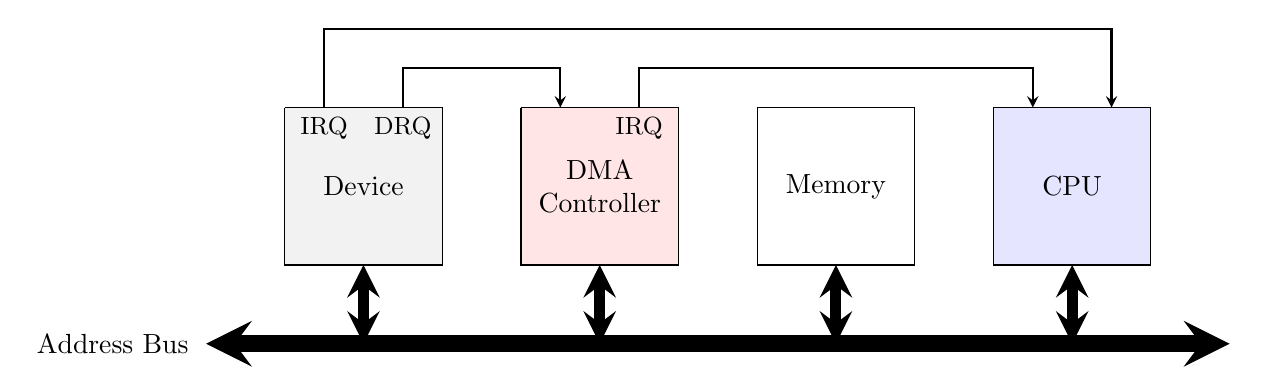
\begin{tikzpicture}
        \draw[fill=gray!10] (0,0) -- (2,0) -- (2,-2) -- (0,-2) -- (0,0);
            \draw (1,-1) node[] {Device};

        \draw[fill=red!10] (3,0) -- (5,0) -- (5,-2) -- (3,-2) -- (3,0);
            \draw[text width=2cm, text centered] (4,-1) node[] {DMA Controller};
    
        \draw (6,0) -- (8,0) -- (8,-2) -- (6,-2) -- (6,0);
            \draw (7,-1) node[] {Memory};

        \draw[fill=blue!10] (9,0) -- (11,0) -- (11,-2) -- (9,-2) -- (9,0);
            \draw (10,-1) node[] {CPU};

        % Draw Arrows
        \draw[darrow, line width=6pt] (-1,-3) node[left] {Address Bus} -- (12,-3);
        \draw[darrow, line width=4pt] (1,-3) -- (1,-2);
        \draw[darrow, line width=4pt] (4,-3) -- (4,-2);
        \draw[darrow, line width=4pt] (7,-3) -- (7,-2);
        \draw[darrow, line width=4pt] (10,-3) -- (10,-2);

        \draw[arrow] (0.5,0) node[below] {\small IRQ} -- (0.5,1) -| (10.5,0);
        \draw[arrow] (1.5,0) node[below] {\small DRQ} -- (1.5,0.5) -| (3.5,0);
        \draw[arrow] (4.5,0) node[below] {\small IRQ} -- (4.5,0.5) -| (9.5,0);
    
    \end{tikzpicture}
\end{center}
\caption{Typical DMA Configuration}
\label{fig:dma-config}
\end{figure}


\subsubsection{DMA Controller}
The DMA controller is a bus mastering device which means it is able to perform read/write operations
independent of the CPU. To perform a I/O to memory DMA the peripheral signals the DMA via an
interrupt, the DMA controller then responds to the peripheral and reads the data. The DMA then uses
the transfer count (TC) register to determine how the number of samples into an allocated memory
section. The DMA then informs the CPU of the completed transfer via interrupt.\\

\noindent The structure of the registers in the DMA are shown in Figure \ref{fig:dma-reg}

\begin{figure}[H]
\begin{center}
    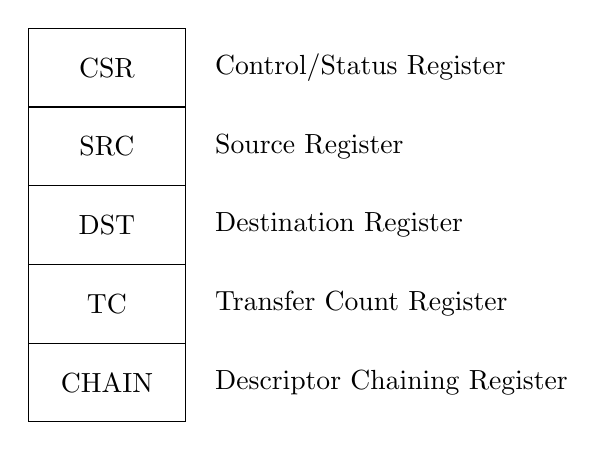
\begin{tikzpicture}
        \draw (0,0) -- (2,0) -- (2,-5) -- (0,-5) -- (0,0);

        \draw (0,-1) -- (2,-1);
        \draw (0,-2) -- (2,-2);
        \draw (0,-3) -- (2,-3);
        \draw (0,-4) -- (2,-4);

        \draw (1,-0.5) node[] {CSR};
        \draw (1,-1.5) node[] {SRC};
        \draw (1,-2.5) node[] {DST};
        \draw (1,-3.5) node[] {TC};
        \draw (1,-4.5) node[] {CHAIN};
    
        \draw (2.25,-0.5) node[right] {Control/Status Register};
        \draw (2.25,-1.5) node[right] {Source Register};
        \draw (2.25,-2.5) node[right] {Destination Register};
        \draw (2.25,-3.5) node[right] {Transfer Count Register};
        \draw (2.25,-4.5) node[right] {Descriptor Chaining Register};
    \end{tikzpicture}
\end{center}
\caption{DMA Controller Register Structure}
\label{fig:dma-reg}
\end{figure}


\subsubsection{DMA Chaining}
DMA's can be chained, this is were the descriptor points to a control block in memory. The control
block is loaded automatically by DMA chaining to start a DMA session. DMA chaining uses a linked
list structure. DMA chaining is shown in Figure \ref{fig:dma-chain}. As the values in the DMA
registers are memory mapped the DMA descriptors can be chained together with pointers. DMA chaining
can be use the achieve a ping pong buffer format, with the second DMA referring to the next buffer
and switching automatically once the transfer count is complete.

\begin{figure}[H]
\begin{center}
    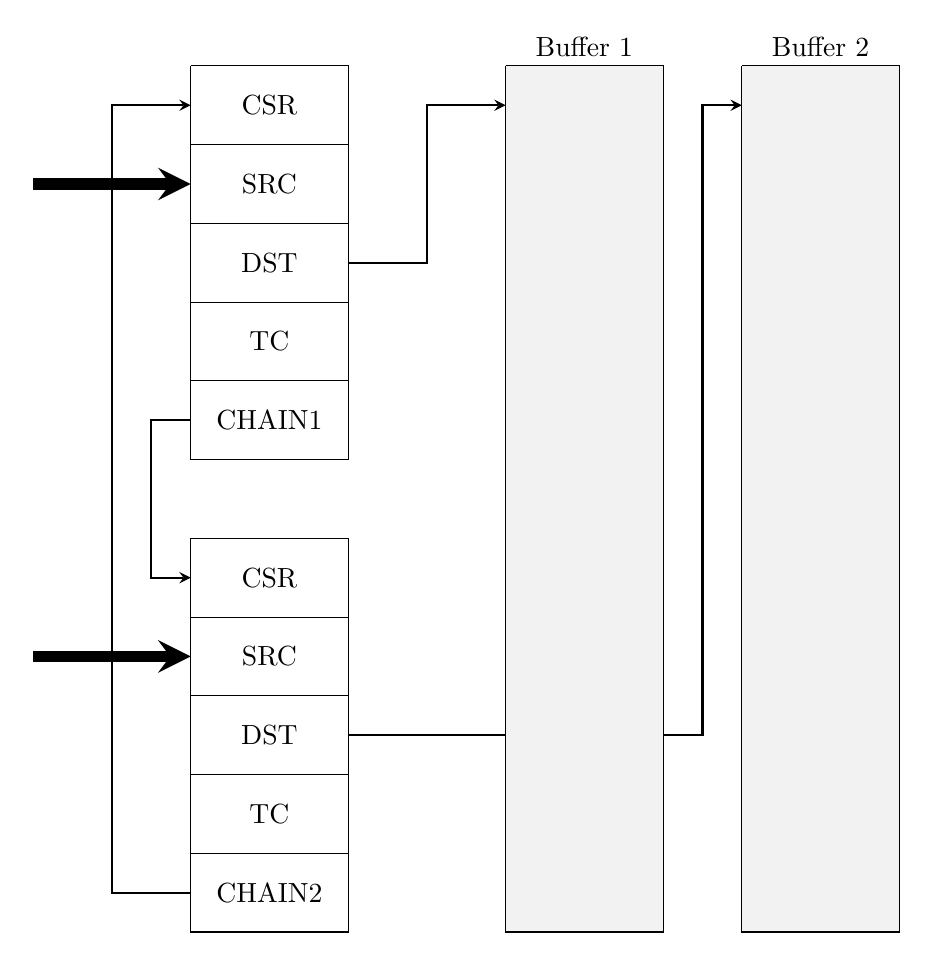
\begin{tikzpicture}
        \draw (0,0) -- (2,0) -- (2,-5) -- (0,-5) -- (0,0);

        \draw (0,-1) -- (2,-1);
        \draw (0,-2) -- (2,-2);
        \draw (0,-3) -- (2,-3);
        \draw (0,-4) -- (2,-4);

        \draw (1,-0.5) node[] {CSR};
        \draw (1,-1.5) node[] {SRC};
        \draw (1,-2.5) node[] {DST};
        \draw (1,-3.5) node[] {TC};
        \draw (1,-4.5) node[] {CHAIN1};
    
        \draw (0,-6) -- (2,-6) -- (2,-11) -- (0,-11) -- (0,-6);

        \draw (0,-7) -- (2,-7);
        \draw (0,-8) -- (2,-8);
        \draw (0,-9) -- (2,-9);
        \draw (0,-10) -- (2,-10);

        \draw (1,-6.5) node[] {CSR};
        \draw (1,-7.5) node[] {SRC};
        \draw (1,-8.5) node[] {DST};
        \draw (1,-9.5) node[] {TC};
        \draw (1,-10.5) node[] {CHAIN2};

        % Draw Arrows
        \draw[arrow] (2,-2.5) -- (3,-2.5) |- (4,-0.5);
        \draw[arrow] (2,-8.5) -- (6.5,-8.5) |- (7,-0.5);

        \draw[fill=gray!10] (4,0) -- (6,0) node[above, midway] {Buffer 1} -- (6,-11) -- (4,-11) -- (4,0);

        \draw[fill=gray!10] (7,0) -- (9,0) node[above, midway] {Buffer 2} -- (9,-11) -- (7,-11) -- (7,0);

        \draw[arrow] (0,-4.5) -- ++(-0.5,0) |- (0,-6.5);
        \draw[arrow] (0,-10.5) -- ++(-1,0) |- (0,-0.5);

        \draw[arrow, line width=4pt] (-2,-1.5) -- (0,-1.5);
        \draw[arrow, line width=4pt] (-2,-7.5) -- (0,-7.5);
    \end{tikzpicture}
\end{center}
\caption{Two-Channel Double Buffered DMA Chaining}
\label{fig:dma-chain}
\end{figure}


\subsubsection{Ping-Pong Buffer}
The Ping Pong buffer, shown in Figure \ref{fig:ping-pong} is a simple buffering system that has two
buffers on the input and output of the processor. This arrangement maximises the processing efficiency
of the processor as data can always be made available and there is always a location to write output
data to.

\begin{figure}[H]
\begin{center}
\begin{adjustbox}{width=\textwidth}
    \begin{circuitikz}
        \draw[fill=red!10] (0,0) -- (2,0) -- (2,-2) -- (0,-2) -- (0,0);
            \draw (1,-1) node[] {\textbf{ADC}};

        \draw[fill=red!10] (3,0) -- (5.5,0) -- (5.5,-2.5) -- (3,-2.5) -- (3,0);
            \draw (4.25,-0.5) node[] {\textbf{BSP}};
            \draw[fill=blue!10] (3.5,-1) -- (5,-1) -- (5,-2) -- (3.5,-2) -- (3.5,-1);
            \draw (4.25, -1.5) node[] {DRR};

        \draw[fill=red!10] (6.5,0) -- (8.5,0) -- (8.5,-2.5) -- (6.5,-2.5) -- (6.5,0);
            \draw(7.5,-1.25) node[] {\textbf{DMA}};

        \draw[fill=red!10] (19,0) -- (21,0) -- (21,-2) -- (19,-2) -- (19,0);
            \draw (20,-1) node[] {\textbf{D/A}};

        \draw[fill=red!10] (15.5,0) -- (18,0) -- (18,-2.5) -- (15.5,-2.5) -- (15.5,0);
            \draw (16.75,-0.5) node[] {\textbf{McBSP2}};
            \draw[fill=blue!10] (16,-1) -- (17.5,-1) -- (17.5,-2) -- (16,-2) -- (16,-1);
            \draw (16.75, -1.5) node[] {DXR};

        \draw[fill=red!10] (12.5,0) -- (14.5,0) -- (14.5,-2.5) -- (12.5,-2.5) -- (12.5,0);
            \draw(13.5,-1.25) node[] {\textbf{DMA2}};


        \draw[fill=gray!30] (3,-4) -- (5,-4) -- (5,-6) -- (3,-6) -- (3,-4);
            \draw[text width=2cm, text centered] (4,-5) node[] {PING IN};
        \draw[fill=gray!10] (3,-7) -- (5,-7) -- (5,-9) -- (3,-9) -- (3,-7);
            \draw[text width=2cm, text centered] (4,-8) node[] {PONG IN};
        
        \draw[fill=gray!30] (16,-4) -- (18,-4) -- (18,-6) -- (16,-6) -- (16,-4);
            \draw[text width=2cm, text centered] (17,-5) node[] {PING OUT};
        \draw[fill=gray!10] (16,-7) -- (18,-7) -- (18,-9) -- (16,-9) -- (16,-7);
            \draw[text width=2cm, text centered] (17,-8) node[] {PONG OUT};

        \draw[fill=red!10] (9,-5.5) -- (12,-5.5) -- (12,-7.5) -- (9,-7.5) -- (9,-5.5);
            \draw (10.5,-6.5) node[] {Processing};
            \draw (10.5,-5.5) node[above] {\textbf{CPU}};
        
        % Switches
        \draw[/tikz/circuitikz/bipoles/length=4cm] (1,-6.5) node[spdt] (insw0) {};
        \draw (insw0.out 1) -- ++(0.3115,0);
        \draw (insw0.out 2) -- ++(0.3115,0);

        \draw[/tikz/circuitikz/bipoles/length=4cm] (7,-6.5) node[rotate=180, spdt] (insw1) {};
        \draw (insw1.out 1) -- ++(-0.3115,0);
        \draw (insw1.out 2) -- ++(-0.3115,0);
        \draw (9,-6.5) -- (insw1.in);
        
        \draw[/tikz/circuitikz/bipoles/length=4cm] (14,-6.5) node[spdt] (outsw0) {};
        \draw (outsw0.out 1) -- ++(0.3115,0);
        \draw (outsw0.out 2) -- ++(0.3115,0);
        \draw (12,-6.5) -- (outsw0.in);

        \draw[/tikz/circuitikz/bipoles/length=4cm] (20,-6.5) node[rotate=180, spdt] (outsw1) {};
        \draw (outsw1.out 1) -- ++(-0.3115,0);
        \draw (outsw1.out 2) -- ++(-0.3115,0);

        % Arrows
        \draw[arrow] (2,-1.5) -- (3.5,-1.5);
        \draw[arrow] (5,-1.5) -- (6.5,-1.5);
        \draw (7.5,-2.5) |- (-2,-3) |- (insw0.in);
        \draw (outsw1.in) -| (23,-3) -| (13.5,-2.5);
        \draw[arrow] (14.5,-1.5) -- (16,-1.5);
        \draw[arrow] (17.5,-1.5) -- (19,-1.5);
    \end{circuitikz}
\end{adjustbox}
\end{center}
\caption{Ping Pong Buffer Configuration}
\label{fig:ping-pong}
\end{figure}



\section{FLASH and Memory}
\subsection{Overview}

\begin{table}[H]
\caption{Embedded Memory Comparison Table}
\label{table:mem-overview}
\begin{center}
\begin{adjustbox} {width=\textwidth}
    \begin{tabular} { | m{2cm} | m{2cm} | m{3cm} | m{2cm} | m{2cm} | m{3cm} | m{3cm} | }
        \hline
        \textbf{Type} & \textbf{Volatile} & \textbf{Writeable} & \textbf{Erase Size} & \textbf{Max
        Erase Cycles} & \textbf{Cost (per Byte)} & \textbf{Speed}\\
        \hline
        \textbf{SRAM} & Yes & Yes & Byte & Unlimited & Expensive & Fast\\
        \textbf{DRAM} & Yes & Yes & Byte & Unlimited & Moderate & Moderate\\
        \textbf{Masked ROM} & No & No & N/A & N/A & Inexpensive & Fast\\
        \textbf{PROM} & No & Once, with programmer & N/A & N/A & Moderate & Fast\\
        \textbf{EPROM} & No & Yes, with programmer & Entire Chip & Limited & Moderate to high & Moderate\\
        \textbf{EEPROM} & No & Yes & Byte & Limited & Expensive & Fast Read, Slow Write \& Erase\\
        \textbf{Flash} & No & Yes & Sector & Limited & Moderate & Fast Read, Slow Write \& Erase\\
        \textbf{NVRAM} & No & Yes & Byte & Unlimited & Expensive (SRAM+Battery) & Fast\\
        \hline
    \end{tabular}
\end{adjustbox}
\end{center}
\end{table}


\subsection{NAND Flash}
A NAND memory cell is a modifed transistor with tunneling based programming. The NAND has the
following array structural elements:

\begin{itemize}
    \item String + Bitline are series connected cells
    \item Wordline is across the cells
    \item Block is the smallest unit to be erased
\end{itemize}

The structure of the NAND Flash is shown in Figure \ref{fig:nand}

\begin{figure}[H]
\begin{center}
    \begin{circuitikz}
        \draw (1,-1) node[nmos] (top0) {};
        \draw (top0.D) -- ++(0,0.5) node[vcc] {} node[above, yshift=0.5cm] {B(0)};
        \draw (1,0) node[jump crossing] (00) {};
        \draw (1,-3) node[pmos] (umid0) {};
        \draw (1,-2) node[jump crossing] (01) {};
        \draw (1,-7) node[pmos] (lmid0) {};
        \draw (1,-6) node[jump crossing] (02) {};
        \draw (1,-9) node[nmos] (bottom0) {};
        \draw (1,-8) node[jump crossing] (03) {};
        \draw (bottom0.S) -- ++(0,-0.5) node[ground] {};

        \draw (3,-1) node[nmos] (top1) {};
        \draw (top1.D) -- ++(0,0.5) node[vcc] {} node[above, yshift=0.5cm] {B(1)};
        \draw (3,0) node[jump crossing] (10) {};
        \draw (3,-3) node[pmos] (umid1) {};
        \draw (3,-2) node[jump crossing] (11) {};
        \draw (3,-7) node[pmos] (lmid1) {};
        \draw (3,-6) node[jump crossing] (12) {};
        \draw (3,-9) node[nmos] (bottom1) {};
        \draw (3,-8) node[jump crossing] (13) {};
        \draw (bottom1.S) -- ++(0,-0.5) node[ground] {};
        
        \draw (5,-1) node[nmos] (top2) {};
        \draw (top2.D) -- ++(0,0.5) node[vcc] {} node[above, yshift=0.5cm] {B(2)};
        \draw (5,0) node[jump crossing] (20) {};
        \draw (5,-3) node[pmos] (umid2) {};
        \draw (5,-2) node[jump crossing] (21) {};
        \draw (5,-7) node[pmos] (lmid2) {};
        \draw (5,-6) node[jump crossing] (22) {};
        \draw (5,-9) node[nmos] (bottom2) {};
        \draw (5,-8) node[jump crossing] (23) {};
        \draw (bottom2.S) -- ++(0,-0.5) node[ground] {};
        
        \draw (11,-1) node[nmos] (top3) {};
        \draw (top3.D) -- ++(0,0.5) node[vcc] {} node[above, yshift=0.5cm] {B(i)};
        \draw (11,-3) node[pmos] (umid3) {};
        \draw (11,-7) node[pmos] (lmid3) {};
        \draw (11,-9) node[nmos] (bottom3) {};
        \draw (bottom3.S) -- ++(0,-0.5) node[ground] {};

        % Draw Lines
        \draw (-1,0) node[left] {DSL} -- (00.west) (00.east) -- (10.west) (10.east) -- (20.west)
        (20.east) -- (5.25,0);
        \draw[dashed] (5.25,0) -- (9.5,0);
        \draw (9.5,0) -| (top3.G);
        \draw (top0.G) -| (0,0) node[circ] {};
        \draw (top1.G) -| (2,0) node[circ] {};
        \draw (top2.G) -| (4,0) node[circ] {};

        \draw (-1,-2) node[left] {WL(j)} -- (01.west) (01.east) -- (11.west) (11.east) -- (21.west)
        (21.east) -- (5.25,-2);
        \draw[dashed] (5.25,-2) -- (9.5,-2);
        \draw (9.5,-2) -| (umid3.G);
        \draw (umid0.G) -| (0,-2) node[circ] {};
        \draw (umid1.G) -| (2,-2) node[circ] {};
        \draw (umid2.G) -| (4,-2) node[circ] {};

        \draw (-1,-6) node[left] {WL(0)} -- (02.west) (02.east) -- (12.west) (12.east) -- (22.west)
        (22.east) -- (5.25,-6);
        \draw[dashed] (5.25,-6) -- (9.5,-6);
        \draw (9.5,-6) -| (lmid3.G);
        \draw (lmid0.G) -| (0,-6) node[circ] {};
        \draw (lmid1.G) -| (2,-6) node[circ] {};
        \draw (lmid2.G) -| (4,-6) node[circ] {};
        
        \draw (-1,-8) node[left] {SSL} -- (03.west) (03.east) -- (13.west) (13.east) -- (23.west) 
        (23.east) -- (5.25,-8);
        \draw[dashed] (5.25,-8) -- (9.5,-8);
        \draw (9.5,-8) -| (bottom3.G);
        \draw (bottom0.G) -| (0,-8) node[circ] {};
        \draw (bottom1.G) -| (2,-8) node[circ] {};
        \draw (bottom2.G) -| (4,-8) node[circ] {};

        \draw (top0.S) -- (01.north) (01.south) -- (umid0.S);
        \draw[dashed] (umid0.D) -- (02.north);
        \draw (02.south) -- (lmid0.S) (lmid0.D) -- (03.north) (03.south) -- (bottom0.D); 
        
        \draw (top1.S) -- (11.north) (11.south) -- (umid1.S);
        \draw[dashed] (umid1.D) -- (12.north);
        \draw (12.south) -- (lmid1.S) (lmid1.D) -- (13.north) (13.south) -- (bottom1.D); 

        \draw (top2.S) -- (21.north) (21.south) -- (umid2.S);
        \draw[dashed] (umid2.D) -- (22.north);
        \draw (22.south) -- (lmid2.S) (lmid2.D) -- (23.north) (23.south) -- (bottom2.D); 

        \draw (top3.S) -- (umid3.S);
        \draw[dashed] (umid3.D) -- (11,-6);
        \draw (11,-6) -- (lmid3.S) (lmid3.D) -- (bottom3.D); 


    \end{circuitikz}
\end{center}
\caption{NAND Flash hardware configuration}
\label{fig:nand}
\end{figure}

To read data a address is placed on the word line and the data is read out from the bit line.

\subsubsection{NOR Based Flash}
The difference between NOR Flash and NAND Flash is in NOR flash every memory cell is directly
connected to the bit line. This results in faster read speeds then NAND but slower write and erase
as well as lower density. For these reasons NOR flash is used in MCU's and NAND is used in USB
drives, SD cards and SATA SSDs. The structure of NOR flash is shown in Figure \ref{fig:nor}.

\begin{figure}[H]
\begin{center}
    \begin{circuitikz}
        \draw (0,0) node[pmos, rotate=-90] (mos0) {};
        \draw (2,0) node[pmos, rotate=-90] (mos1) {};
        \draw (4,0) node[pmos, rotate=-90] (mos2) {};
        \draw (6,0) node[pmos, rotate=-90] (mos3) {};

        \draw (mos0.S) -- (mos1.D) node[ground, midway] {};
        \draw (mos2.S) -- (mos3.D) node[ground, midway] {};
        \draw (mos1.S) -- (mos2.D) node[midway] (helper0) {};
    
        \draw (mos0.G) node[above] {WL(0)};
        \draw (mos1.G) node[above] {WL(1)};
        \draw (mos2.G) node[above] {WL(2)};
        \draw (mos3.G) node[above] {WL(3)};

        \draw (-2,2) node[left] {Bit Line} -- (8,2);
        \draw (mos0.D) -- (mos0.D |- -1,2);
        \draw (mos3.S) -- (mos3.S |- -1,2);
        \draw (3, |- mos0.D) -- (3,2);
    \end{circuitikz}
\end{center}
\caption{NOR Flash Structure}
\label{fig:nor}
\end{figure}


\subsection{Dynamic Memory Allocation}
Dynamic memory allocation using commands like `\textit{malloc()}' and `\textit{free()}' allocate and
deallocate memory from the heap. Dynamic memory presents issues with transparency as local
variables defined by `\textit{malloc()}' are difficult to maintain. `\textit{malloc()}' can also
make embedded software non deterministic under a Real time operating system (RTOS) as memory
allocation time can be slow.

\subsection{Heap Fragmentation}
Heap fragmentation is when the through the process of allocation and freeing the heap gets split
into parts by allocated blocks. These blocks prevent allocation as no contiguous blocks exist due to
the segmented smaller allocated blocks.

\subsection{Global Variables}
Global variables are used to allow access between foreground and background tasks. However, this
makes them \textit{volatile} as they may be changed unexpectedly therefore they cannot be stored in
registers. These global variable must then be stored in RAM, usually SRAM throughout the code run,
this enables faster access to the variable. There are risks with the use of global variables, such
as race conditions some of these risks can be mitigated by using atomic operations (One clock cycle
to complete/cannot be interrupted)

\subsection{Memory Overlays}
Memory overlays are the where different sections of code can be read into internal memory,
overwriting another. This is used to accommodate limited SRAM. To use memory overlays the code/data
must be structured in such a way that not all of the data is required in memory at the same time eg.
code is segmentable or large datasets are not required all at once. Examples of data would be FFT,
Digital filtering and image data. These are represented in C as a `union' an example of an overlay
tree is shown in Figure \ref{fig:overlay}.

\begin{figure}[H]
\begin{center}
\begin{adjustbox} {width=\textwidth}
    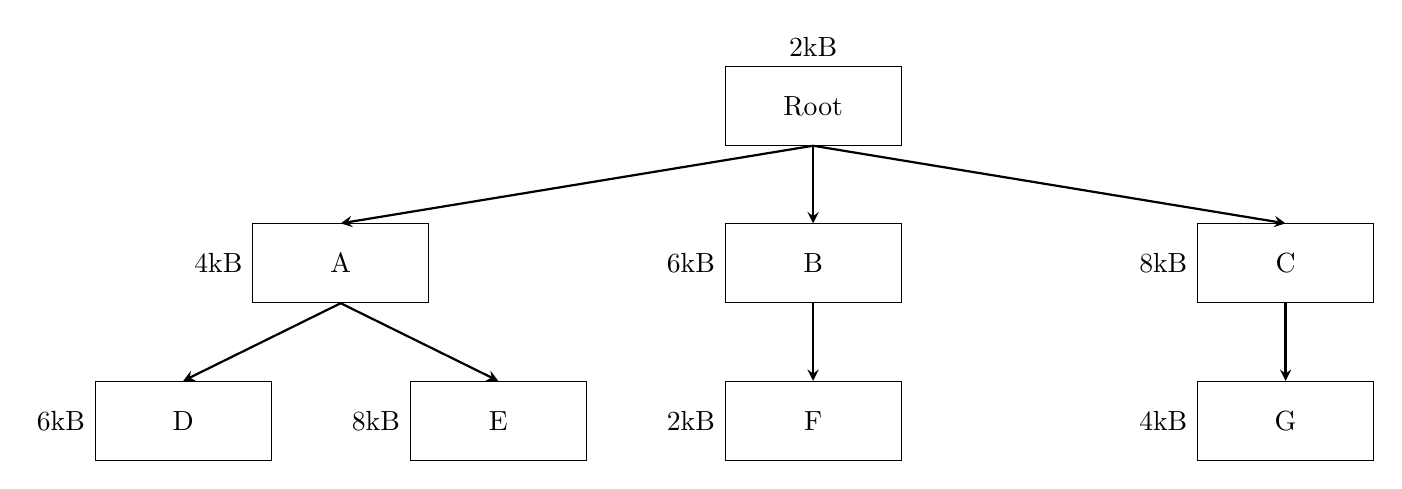
\begin{tikzpicture}
        \node[boxes] (root) {Root};
        \node[boxes, below of=root, xshift=-6cm, yshift=-1cm] (a) {A};
        \node[boxes, below of=root, yshift=-1cm] (b) {B};
        \node[boxes, below of=root, xshift=6cm, yshift=-1cm] (c) {C};
        \node[boxes, below of=a, xshift=-2cm, yshift=-1cm] (d) {D};
        \node[boxes, below of=a, xshift=2cm, yshift=-1cm] (e) {E};
        \node[boxes, below of=b, yshift=-1cm] (f) {F};
        \node[boxes, below of=c, yshift=-1cm] (g) {G};

        \draw (root.north) node[above] {2kB};
        \draw (a.west) node[left] {4kB};
        \draw (b.west) node[left] {6kB};
        \draw (c.west) node[left] {8kB};

        \draw (d.west) node[left] {6kB};
        \draw (e.west) node[left] {8kB};
        \draw (f.west) node[left] {2kB};
        \draw (g.west) node[left] {4kB};

        \draw[arrow] (root.south) -- (a.north);
        \draw[arrow] (root.south) -- (b.north);
        \draw[arrow] (root.south) -- (c.north);
        
        \draw[arrow] (a.south) -- (d.north);
        \draw[arrow] (a.south) -- (e.north);
        \draw[arrow] (b.south) -- (f.north);
        \draw[arrow] (c.south) -- (g.north);

    \end{tikzpicture}
\end{adjustbox}
\end{center}
\caption{Memory Overlay Tree example}
\label{fig:overlay}
\end{figure}


\subsection{Erasing and Writing}
For NAND Flash erasing has to occur by the page. Whereas NOR can erase individual bits. To perform
an erase a large reverse polarity voltage is applied to the floating gate. NAND has to write 
an entire page at a time. NOR's ability to erase/write individual bits increases its random 
read/write speed making it more suitable for RAM (Random Access Memory).

\subsection{Reading}
To read the NAND Flash applies a voltage to the word line and the bit line the voltage is then read
from the bit line to determine the bit state. NOR can read faster than NAND making it suitable for
high speed applications however, it has a lower density then NAND so is not used for large scale
storage such as USB drives.


\section{Delays and Timing}
Delays are used frequently in MCU programming however it is difficult to ensure consistantcy and
accuracy for long delays as interrupts can cause accuracy issues for timers making them unrelaible
for both long time periods and in complicated programs. There will always be a trade off between
time resolution and delay range.

\subsection{Time Resolution and Delay Range}
Delays can have any length, depending on the clock speed of the unit driving it. The
\textit{Granularity} is the measure of a chosen smallest time unit of a delay and the \textit{Range}
is a function the number of core bits/maximum count of a number in an MCU. This range effectively
dictates the maximum time a delay can be, taking into account the granularity and the maximum count
of an MCU.

\begin{table}[H]
\caption{Time resolution and delay range table}
\label{table:time-reso}
\begin{center}
    \begin{tabular} {| m{3cm} | m{3cm} | m{3cm} | m{3cm} | }
        \hline
        Granularity & Range (8-bit) & Range (16-bit) & Range (32-bit)\\
        \hline
        $1\mu \textrm{s}$ & $255\mu \textrm{s}$ & $66\textrm{ms}$ & $1\textrm{min}$\\
        $1\textrm{ms}$ & $255\textrm{ms}$ & $66\textrm{s}$ & $50\textrm{days}$\\
        $1\textrm{s}$ & $4.3\textrm{min}$ & $18\textrm{hr}$ & $136\textrm{yr}$\\
        \hline
    \end{tabular}
\end{center}
\end{table}


To calculate delay length (\ref{eqn:delay}) is used where, $\tau_0$ is the setup delay, $\Delta_tau$
is the timing resolution and $n$ is the number of ticks creating the delay length. The fundimental
tradeoff between delay range and timing resolution under given bit width is shown in
(\ref{eqn:fund-trade-off})

\begin{equation}
    \tau (n) = \tau_0 + n \Delta_\tau
    \label{eqn:delay}
\end{equation}

\begin{equation}
    \tau_{\textrm{max}}=\tau_0 + (2^{M}-1) \Delta_\tau
    \label{eqn:fund-trade-off}
\end{equation}

\subsection{CPU Based Delay}
CPU Based delay is where the CPU clock rates and architecture determine the granularity and delay
range.

\begin{table}[H]
\caption{CPU Clock delay table}
\begin{center}
    \begin{tabular} { | m{3cm} | m{3cm} | m{3cm} |}
        \hline
        CPU Speed & Delay ($1\mu \textrm{s}$) & Delay ($10\mu \textrm{s}$)\\
        \hline
        2MHz & 2 cycles & 20 cycles\\
        20MHz & 20 cycles & 200 cycles\\
        200MHz & 200 cycles & 2000 cycles\\
        2GHz & 2000 cycles & 20000 cycles\\
        \hline
    \end{tabular}
\end{center}
\end{table}


\subsection{Busy Wait/Delay Loops}
Delay Loops are dependent on CPU clock frequency for time resolution as well as architecture for the
delay range. These delay loops run as background tasks which means that the use of them is very
resource intensive on the CPU. This also means that it more accurate for shorter periods.\\

\noindent Busy wait is when a peripheral is `\textit{idle}' initially and waits to either receive data if it is
an input device or receive instructions from the MCU if it is an output device. After data is
received the peripheral starts in `\textit{busy}' state and after completion it moves to a
`\textit{done}' state where it waits for the next instruction. 

\subsection{Timeouts}
Timeouts prevent an embedded system from entering a non-responsive state while waiting for a
particular external event. This is achieved by allowing the system to exit the non-responsive state
after a set amount of time waiting for an external trigger. Eg A temperature sensor reading every 1s
in a case where the sensor is unresponsive and the MCU waits forever for it to respond. To fix this
the MCU may exit the waiting state after a set period to stop issues with the sensor.


\section{Device Drivers}
A device driver is a collection of the functions required to control/use an external device. These
functions include operations such as, Hardware Initialisation, Data access management, interrupt
handling and task management. There drivers can also provide translations for RTOS to hardware.

\begin{itemize}
    \item \textbf{Hardware Startup} - Hardware initialisation upon power-on and reset
    \item \textbf{Hardware Shutdown} - Hardware configuration into its power-off state
    \item \textbf{Hardware Enable/Disable}
    \item \textbf{Hardware Acquire} - Gain locking access to the hardware
    \item \textbf{Hardware Release} - Release locked hardware
    \item \textbf{Hardware Read/Write}
\end{itemize}

\begin{figure}[H]
\begin{center}
    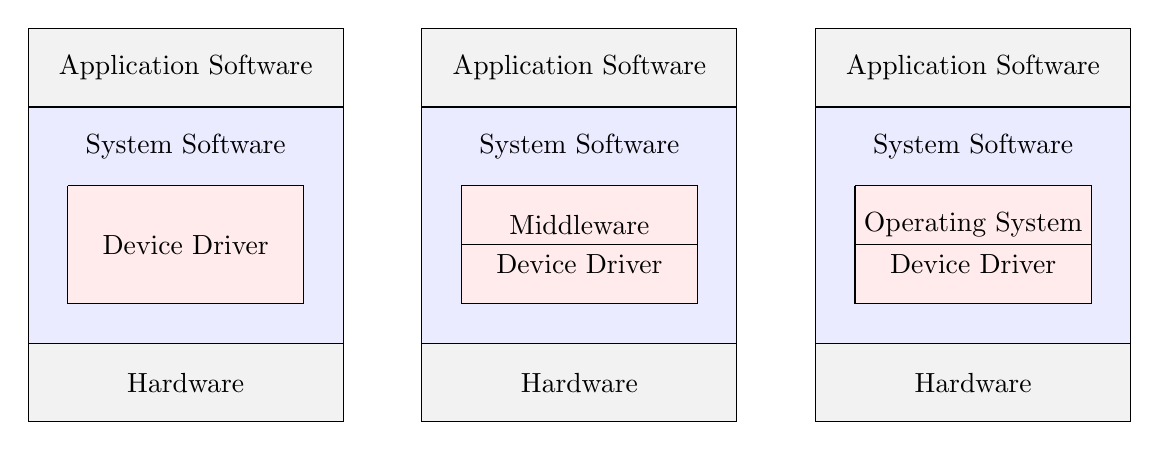
\begin{tikzpicture}
        \draw[fill=gray!10] (0,0) -- (4,0) -- (4,-5) -- (0,-5) -- (0,0);
        \draw[fill=blue!8] (0,-1) -- (4,-1) -- (4,-4) -- (0,-4) -- (0,-1);
        \draw[fill=red!8] (0.5,-2) -- (3.5,-2) -- (3.5,-3.5) -- (0.5,-3.5) -- (0.5,-2);

        \draw[fill=gray!10] (5,0) -- (9,0) -- (9,-5) -- (5,-5) -- (5,0);
        \draw[fill=blue!8] (5,-1) -- (9,-1) -- (9,-4) -- (5,-4) -- (5,-1);
        \draw[fill=red!8] (5.5,-2) -- (8.5,-2) -- (8.5,-3.5) -- (5.5,-3.5) -- (5.5,-2);
        \draw (5.5,-2.75) -- (8.5,-2.75);

        \draw[fill=gray!10] (10,0) -- (14,0) -- (14,-5) -- (10,-5) -- (10,0);
        \draw[fill=blue!8] (10,-1) -- (14,-1) -- (14,-4) -- (10,-4) -- (10,-1);
        \draw[fill=red!8] (10.5,-2) -- (13.5,-2) -- (13.5,-3.5) -- (10.5,-3.5) -- (10.5,-2);
        \draw (10.5,-2.75) -- (13.5,-2.75);

        \draw (2,-0.5) node[] {Application Software};
        \draw (2,-1.5) node[] {System Software};
        \draw (2,-2.75) node[] {Device Driver};
        \draw (2,-4.5) node[] {Hardware};
        
        \draw (7,-0.5) node[] {Application Software};
        \draw (7,-1.5) node[] {System Software};
        \draw (7,-2.5) node[] {Middleware};
        \draw (7,-3) node[] {Device Driver};
        \draw (7,-4.5) node[] {Hardware};
        
        \draw (12,-0.5) node[] {Application Software};
        \draw (12,-1.5) node[] {System Software};
        \draw (12,-2.5) node[] {Operating System};
        \draw (12,-3) node[] {Device Driver};
        \draw (12,-4.5) node[] {Hardware};
    \end{tikzpicture}
\end{center}
\caption{Embedded OSI system models}
\label{fig:embedded-osi}
\end{figure}


\textbf{NOTE}: Middleware is usually used on embedded systems with two or more applications, this
enables flexibility, security, portability, intercommunication and interoperability between
applications.

The advantages and disadvantages of different drivers is shown below:

\begin{itemize}
    \item OS-Supplied Drivers
    \begin{itemize}
        \item {No need to search for compatible drivers}
        \item \red{Only the most popular hardware is supported} 
    \end{itemize}

    \item Manufacturer Supplied Drivers
    \begin{itemize}
        \item {Availability reduces development time}
        \item \red{May not be optimal for a specific application} 
    \end{itemize}
    
    \item Direct Hardware Access
    \begin{itemize}
        \item {Very fast access}
        \item \red{May not take advantage of operating system features} 
    \end{itemize}
    
    \item Third Party Proprietary Driver
    \begin{itemize}
        \item {May add enhanced functionality}
        \item \red{Not avalible for all all operating systems or hardware} 
    \end{itemize}
    
    \item Roll Your Own Driver
    \begin{itemize}
        \item {May be highly optimised for the application}
        \item \red{May require significant development and testing time} 
    \end{itemize}
\end{itemize}

\subsection{Architecture Specific Driver}
Architecture specific drivers use a two layer structure, with the top layer being hardware
independent providing high level commands such as `\textit{uart\_write()}' these commands don't
perform low level operations and are therefore not MCU specific. The bottom layer is known as the
hardware abstraction layer (HAL) and is MCU specific as it directly interacts with hardware
registers.

\subsection{Controls in Drivers}
When designing drivers there are several considerations that need to be made, the first is regarding
errors, eg. `\textit{malloc()}' on failure returns \textit{NULL}, this indicates an error such as
insufficient memory. There are two conventional options for return types the first is, a small
integer eg. `-1' the second is a pointer. The advantages of using a small integer is that is is easy
to check and the disadvantage is that a mapping table is required. For pointers the advantage is
that it is faster as there is no table lookup and the disadvantage is that more memory is used.\\

\noindent Next the device needs a handle, used to specify the appropriate device.\\

\noindent Next is data passing, for this passing a pointer is typical\\

\noindent The most important factor however, is consistency for each of these components.

\subsection{Configuration Parameters}
There are two methods for passing configuration parameters to a device driver. The first is using a
static configuration, this is when the parameters are passed at compile time. This method is simple
how can become difficult to maintain. To create a static configuration macros, enums, header
definitions and conditional compilation can be used (compile options eg.
architecture). The second method is dynamic configuration, this is where the driver parameter
structures are passed into setup type functions at run-time, this model is used extensively for high
level languages. These configuration structures can be stored as an object library in an include
or object file.

\subsection{Performance Considerations}
Overall, the performance of the drivers is dependent on the hardware used. There are two main
operation type, the first is interrupt operation. This operation type is relatively low latency,
these interrupts can be software generated, external (based on pin change) or internal (DMA,
internal peripheral etc.). Using interrupts can result in components of the software being
non-deterministic as interrupts, especially ones on an external trigger can be unpredictable. The
second operation type is to use polling, this method is simple however can be very CPU intensive.
Polling is often integrated with RTOS.

\subsection{Multiple Devices}
To work with multiple devices the code must be `reentrant' this is when code returns to were it
started and doesn't move to a different one. This means that setting a global state then writing
will have issues whereas passing the value of a device to be written to/read from into the
read/write function.



\section{DSP}
Digital Signal Processing (DSP) does performs signal processing in the digital domain. This approach
is simpler than analog signal processing. This sort of processing is well suited for speech and
language processing, image processing etc.

\subsection{System Design Considerations}
\subsubsection{Hardware}
When selecting hardware ensure that the DSP has the appropriate fixed/floating point data unit,
adequate data width and processing speed for the desired application. Also the sampling rate may be
either fixed or variable. The available interfaces are important, such as serial and parallel
interface compatibility. Finally the memory types are an important consideration for hardware
selection.

\subsubsection{Software}
When making software design decisions ensure the appropriate language/group of languages are used to
best fit the desired use case. Also consider any operating systems and any debugging or testing
toolchains that may be required.\\

\noindent DSP's are best suited for low complexity/high sample rate data collection and processing.

\begin{table}[H]
\caption{MCU vs. DSP Comparison Table}
\label{table:mcu-v-dsp}
\begin{center}
    \begin{tabular} { | m{4cm} | m{4cm} | m{4cm} | }
        \hline
        \empty & Microcontrollers (MCUs) & Digital Signal Processors\\
        \hline
        Functionality & General purpose, more suitable for sensing and control applications & More
        specialised, architecture and instruction set more suitable for signal processing\\
        \hline
        Power Consumption & Suitable for very low power applications & Typically run at full power\\
        \hline
        On-chip Peripherals & Typically have extensive inbuilt support & Most peripherals are not
        supoorted\\
        \hline
        Architecture & RISC-based with high performance extensions & Optimised instruction and
        architecture for executing repetitive algorithms\\
        \hline
        Ease of Use & Short development with good documentation and tools & Longer development time
        as there is more of an optimisation focus\\
        \hline

    \end{tabular}
\end{center}
\end{table}


\subsection{Common DSP Features}
DSP's usually have features such as, multiple bus architectures eg. Harvard, modified Harvard etc.,
fast multiply and accumulate (MAC) and dot product processing. Typically DSP's also execute one
instruction per cycle and have very fast clock rates. Also present are special address modes eg.
circular addressing, specialised execution and control (no loop overhead, and a delayed branch
instruction) and specialised peripherals \& I/O devices eg. communications between DSP and CODECs,
multiple channel serial interfaces and DMA modules. Solutions such as DSP+ARM exist, with is a
combination of ARM core/s for command and control and a DSP for real-time processing.

\subsection{MAC}
Multiply and accumulate (MAC) is a core DSP operation and hence must be very efficient examples of
multiply and accumulate functions are:

\begin{itemize}
    \item Convolution
    \item Correlation (Auto and Cross)
    \item Fourier and Inverse Fourier transforms
    \item $c_{i}=\sum_{k=0}^{N}a_{i} \dot b_{i}$
    \item Digital/adaptive filtering
    \item Neural Networks
\end{itemize}

DSP's typically have dedicated MAC modules to enable extreemly efficent MAC an example of this is
shown in Figure \ref{fig:mac-unit}.

\begin{figure}[H]
\begin{center}
    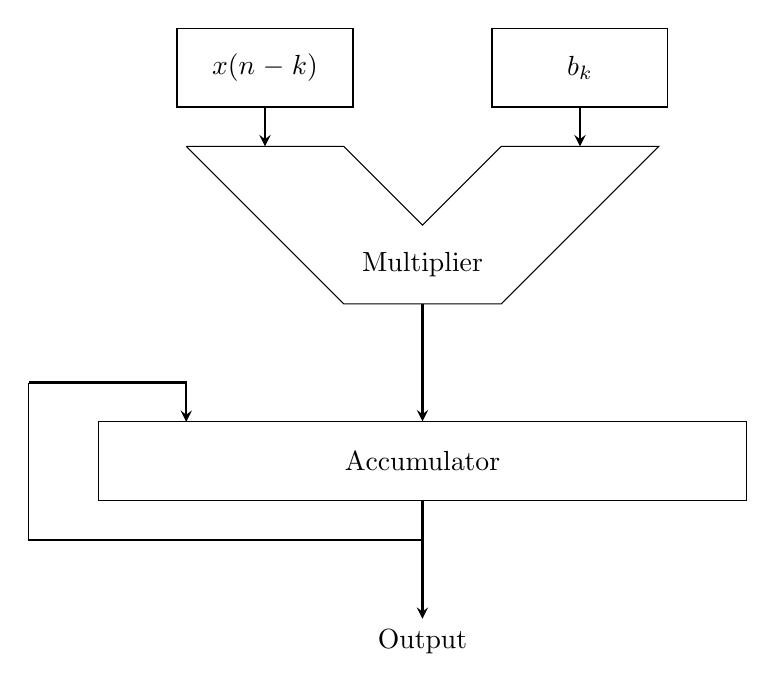
\begin{tikzpicture}
        \draw (0,-1) node[boxes] (m0) {$x(n-k)$};
        \draw (4,-1) node[boxes] (m1) {$b_k$};
        \draw (-1,-2) -- (1,-2) -- (2,-3) -- (3,-2) -- (5,-2) -- (3,-4) -- (1,-4) --
        (-1,-2);

        \draw (2,-3.5) node[] {Multiplier};

        \draw (2,-6) node[xwboxes] (acc) {Accumulator};

        % Arrows
        \draw[arrow] (m0.south) -- (0,-2);
        \draw[arrow] (m1.south) -- (4,-2);

        \draw[arrow] (2,-4) -- (acc.north);
        \draw[arrow] (acc.south) -- (2,-8) node[below] {Output};
        \draw (2,-7) -| (-3,-5);
        \draw[arrow] (-3,-5) -| (-1,-5.5);
    \end{tikzpicture}
\end{center}
\caption{DSP Multiply and Accumulate (MAC) Module}
\label{fig:mac-unit}
\end{figure}


\subsubsection{FIR Filtering}
Finite Impulse Response filtering (FIR) is a digital filtering method, an execution of which can be
found in Figure \ref{fig:fir-dsp}

\begin{figure}[H]
\begin{center}
\begin{adjustbox} {width=\textwidth}
    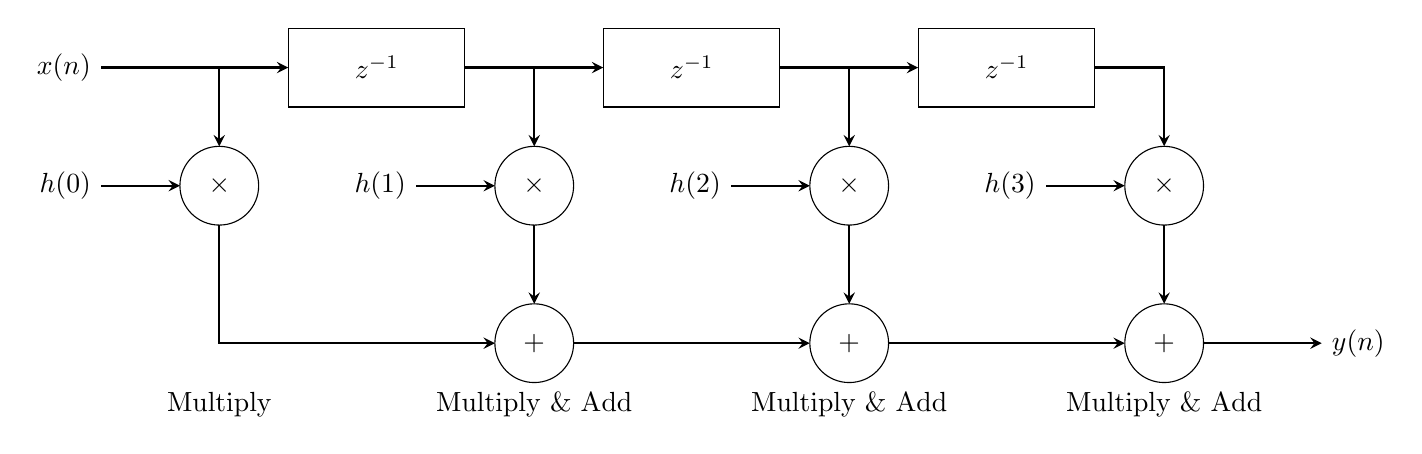
\begin{tikzpicture}
        \draw (2,0) node[boxes] (z0) {$z^{-1}$} (6,0) node[boxes] (z1) {$z^{-1}$} (10,0) node[boxes]
        (z2) {$z^{-1}$};

        \draw (0,-1.5) circle (0.5cm);
        \draw[arrow] (-1.5,-1.5) node[left] {$h(0)$} -- (-0.5,-1.5);
        \draw (0,-1.5) node[] {$\times$};

        \draw (4,-1.5) circle (0.5cm);
        \draw[arrow] (2.5,-1.5) node[left] {$h(1)$} -- (3.5,-1.5);
        \draw (4,-1.5) node[] {$\times$};
        \draw (4,-3.5) circle (0.5cm);
        \draw (4,-3.5) node[] {$+$};

        \draw (8,-1.5) circle (0.5cm);
        \draw[arrow] (6.5,-1.5) node[left] {$h(2)$} -- (7.5,-1.5);
        \draw (8,-1.5) node[] {$\times$};
        \draw (8,-3.5) circle (0.5cm);
        \draw (8,-3.5) node[] {$+$};

        \draw (12,-1.5) circle (0.5cm);
        \draw[arrow] (10.5,-1.5) node[left] {$h(3)$} -- (11.5,-1.5);
        \draw (12,-1.5) node[] {$\times$};
        \draw (12,-3.5) circle (0.5cm);
        \draw (12,-3.5) node[] {$+$};

        \draw[arrow] (-1.5,0) node[left] {$x(n)$} -- (z0.west); 
        \draw[arrow] (-1.5,0) -| (0,-1);
        \draw[arrow] (0,-2) |- (3.5,-3.5);

        \draw[arrow] (z0.east) -- (z1.west);
        \draw[arrow] (z0.east) -| (4,-1);
        \draw[arrow] (4,-2) -- (4,-3);

        \draw[arrow] (z1.east) -- (z2.west);
        \draw[arrow] (z1.east) -| (8,-1);
        \draw[arrow] (8,-2) -- (8,-3);

        \draw[arrow] (z2.east) -| (12,-1);
        \draw[arrow] (12,-2) -- (12,-3);
        
        \draw[arrow] (4.5,-3.5) -- (7.5,-3.5);
        \draw[arrow] (8.5,-3.5) -- (11.5,-3.5);
        \draw[arrow] (12.5,-3.5) -- (14,-3.5) node[right] {$y(n)$};
        
        \draw (0,-4) node[below] {Multiply};
        \draw (4,-4) node[below] {Multiply \& Add};
        \draw (8,-4) node[below] {Multiply \& Add};
        \draw (12,-4) node[below] {Multiply \& Add};
    \end{tikzpicture}
\end{adjustbox}
\end{center}
\caption{FIR Filter DSP Operations}
\label{fig:fir-dsp}
\end{figure}


This results in the following operations:

\begin{center}
\begin{tabular} {l l l}
    Fir: & IN & PORTX\\
    & MPY & *x-, *h+,AC0\\
    & MAC & *x-, *h+,AC0\\
    & MAC & *x-, *h+,AC0\\
    & MAC & *x-, *h+,AC0\\
    & MAC & *x-, *h+,AC0\\
    & OUT & PORTY
\end{tabular}
\end{center}

\subsection{Fixed Point Data}
In a fixed point DSP data is represented by a binary fraction $\in (-1, 1)$ this method reduces the
dynamic range for multiplication eg. $0.9\times 0.9 = 0.81$ to maintain the original bit width the
output value is concatenated to $0.8$ to encode the numbers two compliment is used as it allows sign
coding. When multiplying negative values `1's are appended to the front. The result is output in
two's compliment.

\noindent The binary mapping to decimal values are:
\begin{equation}
\begin{bmatrix}
    -1 & \frac{1}{2} & \frac{1}{4} & \frac{1}{8}\\
\end{bmatrix}
\end{equation}

\begin{equation}
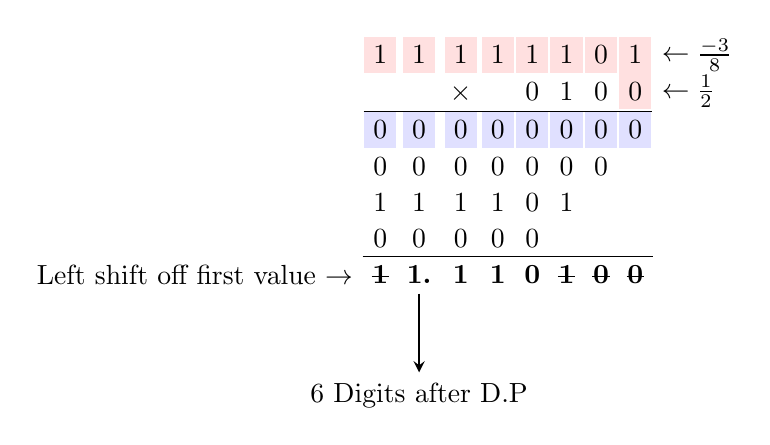
\begin{tikzpicture}[baseline={([yshift=-.5ex]current bounding box.center)}]
    \node[matrix of math nodes] (fixed) {
        \node[fill=red!12](fixed-1-1){1};&\node[fill=red!12]{1};&\node[fill=red!12]{1};&\node[fill=red!12]{1};&
        \node[fill=red!12]{1};&\node[fill=red!12]{1};&\node[fill=red!12]{0};&\node[fill=red!12](fixed-1-8){1};\\
        \empty & \empty & \times & \empty & 0&1&0&\node[fill=red!12](fixed-2-8){0};\\
        \node[fill=blue!12](fixed-3-1){0};&\node[fill=blue!12]{0};&\node[fill=blue!12]{0};&\node[fill=blue!12]{0};&
           \node[fill=blue!12]{0};&\node[fill=blue!12]{0};&\node[fill=blue!12]{0};&\node[fill=blue!12](fixed-3-8){0};\\
        0&0&0&0&0&0&0\\
        1&1&1&1&0&1\\
        0&0&0&0&0\\
        \textbf{\sout{1}}&\textbf{1.}&\textbf{1}&\textbf{1}&\textbf{0}&\textbf{\sout{1}}&\textbf{\sout{0}}&\textbf{\sout{0}}\\
    };
    \draw (fixed-1-8.east) node[right] {$\gets \frac{-3}{8}$};
    \draw (fixed-2-8.east) node[right] {$\gets \frac{1}{2}$};
    \draw (fixed-7-1.west) node[left] {Left shift off first value $\to$};
    \draw (fixed-3-1.north west) -- (fixed-3-8.north east); 
    \draw (fixed-7-1.north west) -- (fixed-7-8.north east);
    \draw[arrow] (fixed-7-2.south) -- ++(0,-1) node[below] {6 Digits after D.P};
\end{tikzpicture}
\label{eqn:fixed-point}
\end{equation}

The following fixed point calculation is $\frac{3}{8} \times \frac{1}{4}$

\begin{equation}
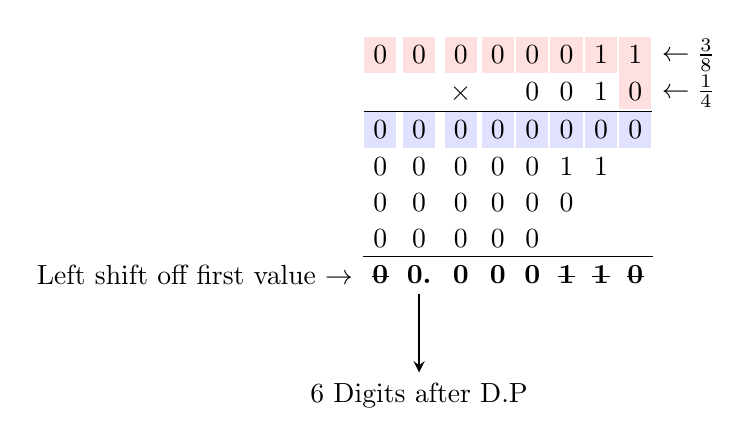
\begin{tikzpicture}[baseline={([yshift=-.5ex]current bounding box.center)}]
    \node[matrix of math nodes] (fixed) {
        \node[fill=red!12](fixed-1-1){0};&\node[fill=red!12]{0};&\node[fill=red!12]{0};&\node[fill=red!12]{0};&
            \node[fill=red!12]{0};&\node[fill=red!12]{0};&\node[fill=red!12]{1};&\node[fill=red!12](fixed-1-8){1};\\
        \empty & \empty & \times & \empty & 0&0&1&\node[fill=red!12](fixed-2-8){0};\\
        \node[fill=blue!12](fixed-3-1){0};&\node[fill=blue!12]{0};&\node[fill=blue!12]{0};&\node[fill=blue!12]{0};&
           \node[fill=blue!12]{0};&\node[fill=blue!12]{0};&\node[fill=blue!12]{0};&\node[fill=blue!12](fixed-3-8){0};\\
        0&0&0&0&0&1&1\\
        0&0&0&0&0&0\\
        0&0&0&0&0\\
        \textbf{\sout{0}}&\textbf{0.}&\textbf{0}&\textbf{0}&\textbf{0}&\textbf{\sout{1}}&\textbf{\sout{1}}&\textbf{\sout{0}}\\
    };
    \draw (fixed-1-8.east) node[right] {$\gets \frac{3}{8}$};
    \draw (fixed-2-8.east) node[right] {$\gets \frac{1}{4}$};
    \draw (fixed-7-1.west) node[left] {Left shift off first value $\to$};
    \draw (fixed-3-1.north west) -- (fixed-3-8.north east); 
    \draw (fixed-7-1.north west) -- (fixed-7-8.north east); 
    \draw[arrow] (fixed-7-2.south) -- ++(0,-1) node[below] {6 Digits after D.P};
\end{tikzpicture}
\label{eqn:fixed-point0}
\end{equation}


The following fixed point calculation is $\frac{5}{8} \times \frac{1}{2}$

\begin{equation}
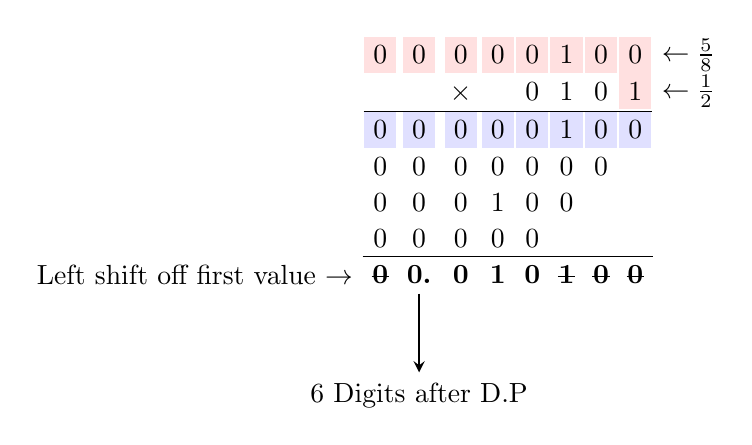
\begin{tikzpicture}[baseline={([yshift=-.5ex]current bounding box.center)}]
    \node[matrix of math nodes] (fixed) {
        \node[fill=red!12](fixed-1-1){0};&\node[fill=red!12]{0};&\node[fill=red!12]{0};&\node[fill=red!12]{0};&
            \node[fill=red!12]{0};&\node[fill=red!12]{1};&\node[fill=red!12]{0};&\node[fill=red!12](fixed-1-8){0};\\
        \empty & \empty & \times & \empty & 0&1&0&\node[fill=red!12](fixed-2-8){1};\\
        \node[fill=blue!12](fixed-3-1){0};&\node[fill=blue!12]{0};&\node[fill=blue!12]{0};&\node[fill=blue!12]{0};&
           \node[fill=blue!12]{0};&\node[fill=blue!12]{1};&\node[fill=blue!12]{0};&\node[fill=blue!12](fixed-3-8){0};\\
        0&0&0&0&0&0&0\\
        0&0&0&1&0&0\\
        0&0&0&0&0\\
        \textbf{\sout{0}}&\textbf{0.}&\textbf{0}&\textbf{1}&\textbf{0}&\textbf{\sout{1}}&\textbf{\sout{0}}&\textbf{\sout{0}}\\
    };
    \draw (fixed-1-8.east) node[right] {$\gets \frac{5}{8}$};
    \draw (fixed-2-8.east) node[right] {$\gets \frac{1}{2}$};
    \draw (fixed-7-1.west) node[left] {Left shift off first value $\to$};
    \draw (fixed-3-1.north west) -- (fixed-3-8.north east); 
    \draw (fixed-7-1.north west) -- (fixed-7-8.north east); 
    \draw[arrow] (fixed-7-2.south) -- ++(0,-1) node[below] {6 Digits after D.P};
\end{tikzpicture}
\label{eqn:fixed-point0}
\end{equation}


\subsubsection{Programming} Programming a DSP can be much more efficient in ASM (Assembly) in terms of
both memory and execution time when compared to C


\section{Data Acquisition}
Data acquisition can take many forms, nd measure a huge range of effects/properties eg. Voltage,
current, light intensity etc. One of the most common data acquisition components is an ADC. There
are several common ADC types including Flash, Sigma-Delta ($\sum-\Delta$), CODECs, Successive
approximation and integrating ADCs.

\subsection{Ideal v. Practical Sampling}
Ideal sampling would have an input signal which would be sampled using convultion with a time domain
driac comb (series of delta functions) offset by the sample interval $f(x)=\sum_{k=0}^N \delta(x-k)$.
However, this is not realisable as a voltage impulse cannot be created without an $\infty$ current
therefore the sampling waveform looks more similar to a low duty cycle pulse signal with a pulse
width of $T_0$ and a sampling period of $T_s=1/2W$

\subsection{Uniform Quantisation}
An N-bit uniform quantisation has $2^N$ levels to match a continuos input analog voltage to a
quantised digital output.

\begin{itemize}
    \item Quantisation Interval: $\Delta = (V_{\textrm{max}} - V_{\textrm{min}})/2^N$
    \item Quantisation Error: $V_{err} \in [-\Delta / 2, \Delta / 2]$
    \item Variance of Error: $\Delta ^2/12$ 
    \item SNR: $10log_{10} (\frac{(V_{\textrm{max}}-V_{\textrm{min}})^2/8}{\Delta ^2/12}$)
\end{itemize}

\subsection{FLASH Quantisation}
FLASH Quantisation uses a resistor ladder and comparators to determine the analog input voltage of a
signal. This type of quantisation is the fastest however the accuracy is poor. The structure of a
FLASH quantiser is shown in Figure \ref{fig:flash-quant}.

\begin{figure}[H]
\begin{center}
    \begin{circuitikz}
        \draw (0,0) node[op amp] (op0) {};
        \draw (0,-4) node[op amp] (op1) {};
        \draw (0,-8) node[op amp] (op2) {};
        \draw (0,-12) node[op amp] (op3) {};

        \draw (op0.-) -| (-2, 0.5) to[R=R] (-2,-3.5) node[circ]{} |- (op1.-);
        \draw (-2, -3.5) to[R=R] (-2,-7.5) node[circ]{} |- (op2.-);
        \draw (-2, -7.5) to[R=R] (-2,-11.5) node[circ]{} |- (op3.-);
        \draw (-2, -11.5) to[R=R] (-2,-15.5) node[rground]{};
        \draw (-2,4.5) to[R=R] (-2, 0.5);
        \draw (-2,4.5) node[rground, rotate=180] {};

        \draw (-3,-7) node[left] {Analog In} -- (-1.5,-7);
        \draw (-1.5,-7) -| (op0.+);
        \draw (-1.5,-7 -| op1.+) node[circ] {};
        \draw (-1.5,-7) -| (op3.+);
        \draw (op1.+) node[circ] {};
        \draw (op2.+) node[circ] {};

        \draw (4,-6) node[dipchip, num pins=8, hide numbers, no topmark,
            external pins width=0](decoder) {};
        \draw (4,-6) node[rotate=90] {Decoder};

        \draw (decoder.bpin 1) -- ++(-0.5,0) |- (op0.out);
        \draw (decoder.bpin 2) -- ++(-1,0) |- (op1.out);
        \draw (decoder.bpin 3) -- ++(-1,0) |- (op2.out);
        \draw (decoder.bpin 4) -- ++(-0.5,0) |- (op3.out);
    \end{circuitikz}
\end{center}
\caption{4-bit FLASH Quantiser Structure}
\label{fig:flash-quant}
\end{figure}


\subsection{Sigma-Delta ADC ($\sum - \Delta$ ADC)}
The sigma-delta ($\sum - \Delta$) ADC is uses summing and integration to determine the value of the
analog input. This significantly decreases the effect of quantisation noise as it acts as high pass
filter for the noise, skewing it into higher frequencies outside of the digital filter passband. A
block diagram for the sigma delta ADC is shown in Figure \ref{fig:sig-delt}.

\begin{figure}[H]
\begin{center}
\begin{adjustbox} {width=\textwidth}
    \begin{circuitikz}
        \draw (0,0) circle (1cm);
        \draw (-1.5,-0.5) node[] {\textbf{\large $+$}};
        \draw (-0.5,-1.5) node[] {\textbf{\large $-$}};
        \draw (0,0) node[] (sig) {\huge $\sum$};
        \draw (4,0) node[square] (int) {\huge $\int$};

        \draw (8,0) node[square] (adc) {\large 1-bit ADC};
        \draw (14,0) node[square, minimum width=3cm, text width=3cm] (ddf) {\large Digital Decimation Filter};

        \draw (6,-4) node[square] (dac) {\large 1-bit DAC};
        \draw[arrow, line width=2pt] (-2,0) node[left] {\large Analog Input} -- (-1,0);
        \draw[arrow, line width=2pt] (1,0) -- (int.west);
        \draw[arrow, line width=2pt] (int.east) -- (adc.west);
        \draw[arrow, line width=2pt] (adc.east) -- (ddf.west);
        \draw[arrow, line width=2pt] (ddf.west) ++(-2,0) node[circ]{} |- (dac.east);
        \draw[arrow, line width=2pt] (dac.west) -| (0,-1);

        \draw[arrow, line width=2pt] (ddf.east) -- ++(2,0) node[right] {\large Digital Output};
    
    \end{circuitikz}
\end{adjustbox}
\end{center}
\caption{Sigma-Delta ($\sum \Delta$) ADC block diagram}
\label{fig:sig-delt}
\end{figure}


\subsubsection{Importance of Oversampling}
Sigma Delta ADC's must oversample to ensure accuracy of data collection eg. if not oversampling
enough there cannot be a distinction between different rates of change. This occurs when the slopes
are extremely steep causing the Sigma Delta to fall behind in its estimate if many of these high
frequency changes occur the ADC can experience issues with increasing error.

\subsubsection{Digital Filter}
The Digital Decimation Filter performs digital low pass filtering on the output signal, this removes
all of the high frequency quantisation noise and leaves just the output bit stream.

\subsubsection{Noise Shaping}
The integrator acts a high pass filter for the noise, therefore it pushes the noise into higher
frequencies. This noise is then able to be removed in the digital filtering stage.



\end{document}
